%%%%%%%%%%%%%%%%%%%%%%%%%%%%%%%%%%%%%%%%%%%%%%%%%%%%%%%%%%%%%%%%%%%%%%%%%%%%%%%%
% \documentclass[t]{beamer}
\usepackage[
    orientation=landscape,
    size=custom,
    width=25.4,
    height=19.05,
    scale=0.63 % erzeugt 16pt Schriftgröße
]{beamerposter}

\newcommand{\PraesentationSchriftgroesseSehrGross}{\fontsize{30}{45}}
\newcommand{\PraesentationSchriftgroesseGross}{\fontsize{22}{33}}
\newcommand{\PraesentationSchriftgroesseNormal}{\fontsize{16}{29}}
\newcommand{\PraesentationSchriftgroesseKlein}{\fontsize{12}{18}}
\newcommand{\PraesentationSchriftgroesseDreizeiler}{\fontsize{7}{10}}
\newcommand{\PraesentationSchriftgroesseAufzaehlungszeichen}{\fontsize{10}{8}}

\newcommand{\PraesentationAbstandAbsatz}{22.1pt}
\newcommand{\PraesentationPositionKorrekturOben}{0cm}
\newcommand{\PraesentationBeispieleSchriftgroessen}{30 | 22 | 16 | 12}
\input{./Ressourcen/Praesentation/Praeambel.tex} % Layout 4:3
%\documentclass[aspectratio=169]{beamer}
\documentclass[t,aspectratio=169]{beamer}
\usepackage[
    orientation=landscape,
    size=custom,
    width=25.4,
    height=14.2875,
    scale=0.5
]{beamerposter}

\newcommand{\PraesentationSchriftgroesseSehrGross}{\fontsize{25}{38}}
\newcommand{\PraesentationSchriftgroesseGross}{\fontsize{18}{27}}
\newcommand{\PraesentationSchriftgroesseNormal}{\fontsize{14}{21}}
\newcommand{\PraesentationSchriftgroesseKlein}{\fontsize{11}{17}}
\newcommand{\PraesentationSchriftgroesseDreizeiler}{\fontsize{7}{10}}
\newcommand{\PraesentationSchriftgroesseAufzaehlungszeichen}{\fontsize{10}{8}}

\newcommand{\PraesentationAbstandAbsatz}{18pt}
\newcommand{\PraesentationPositionKorrekturOben}{-1cm}
\newcommand{\PraesentationBeispieleSchriftgroessen}{25 | 18 | 14 | 11}
\usepackage[utf8]{inputenc}
\usepackage[T1]{fontenc} % Zeichensatzkodierung

\usepackage{calc} % Berechnungen

\usepackage{relsize}
\usepackage{xspace}
\usepackage{listings}

%\usepackage[ngerman]{babel} % Deutsche Lokalisierung
\usepackage{graphicx} % Grafiken
\graphicspath{ {./Assets/} }
\usepackage{caption,setspace}
\usepackage[export]{adjustbox}
\usepackage[absolute, overlay]{textpos} % Positionierung
% Silbentrennung:
\usepackage{hyphenat}
%\tolerance 2414
%\hbadness 2414
%\emergencystretch 1.5em
%\hfuzz 0.3pt
%\widowpenalty=10000     % Hurenkinder
%\clubpenalty=10000      % Schusterjungen
%\vfuzz \hfuzz

% Euro-Symbol:
\usepackage[gen]{eurosym}
\DeclareUnicodeCharacter{20AC}{\euro{}}

% Schriftart Helvetica:
\usepackage[scaled]{helvet}
\renewcommand{\familydefault}{\sfdefault}

\usepackage{mathptmx} % skalierbare Formelschriften

\usepackage{tabularx}

\usepackage{multicol} % mehrspaltiger Text


\usepackage{tikz}
\usetikzlibrary{arrows.meta,decorations.markings,calc,shapes.geometric,shadows,arrows,patterns}
\usepackage{pgfplots}
\usepackage{pgfplotstable}


\usepackage{amsmath}
\usepackage{amssymb}
\usepackage{amsfonts}
\usepackage{amsthm}
\newtheorem*{thm}{Theorem}
\newtheorem*{dfn}{Definition}
\newtheorem*{lma}{Lemma}
\usepackage{mathtools}
\usepackage{xfrac}
\usepackage{siunitx}
\usepackage{commath}
\usepackage{marvosym}
\DeclareMathAlphabet{\mathcal}{OMS}{cmsy}{m}{n}

\DeclareMathOperator*{\argmax}{arg\,max}
\DeclareMathOperator*{\argmin}{arg\,min}
\DeclareMathOperator*{\esssup}{ess\,sup}

\newcommand*{\logeq}{\ratio\Leftrightarrow}

% Erweiterbare Fusszeile:
\newcommand{\PraesentationFusszeileZusatz}{}

% Define TUM corporate design colors
% Taken from http://portal.mytum.de/corporatedesign/index_print/vorlagen/index_farben
\definecolor{TUMBlue}{HTML}{0065BD}
\definecolor{TUMSecondaryBlue}{HTML}{005293}
\definecolor{TUMSecondaryBlue2}{HTML}{003359}
\definecolor{TUMBlack}{HTML}{000000}
\definecolor{TUMWhite}{HTML}{FFFFFF}
\definecolor{TUMDarkGray}{HTML}{333333}
\definecolor{TUMGray}{HTML}{808080}
\definecolor{TUMLightGray}{HTML}{CCCCC6}
\definecolor{TUMAccentGray}{HTML}{DAD7CB}
\definecolor{TUMAccentOrange}{HTML}{E37222}
\definecolor{TUMAccentGreen}{HTML}{A2AD00}
\definecolor{TUMAccentLightBlue}{HTML}{98C6EA}
\definecolor{TUMAccentBlue}{HTML}{64A0C8}


\newcommand{\LL}{\mathcal{L}}
\newcommand{\RR}{\mathcal{R}}
\newcommand{\repof}{\mathrm{rep\_of}_\mathcal{L}\,}
\newcommand{\ufabstart}{\mathrm{ufa\_}\beta\mathrm{\_start}_\mathcal{L}}
\newcommand{\ufabtrans}{\mathrm{ufa\_}\beta^+_\mathcal{L}}
\newcommand{\ufabrefl}{\mathrm{ufa\_}\beta^*_\mathcal{L}}
\newcommand{\ufaalpha}{\mathrm{ufa\_}\alpha_\mathcal{L}}
\newcommand{\level}{\mathrm{level}_{\LL,\RR}\,}
\newcommand{\iindex}{\mathrm{index}_{\LL,\RR}\,}
\newcommand{\philr}{\phi\, \LL\, \RR\,}
\newcommand{\philrb}{\phi\, \LL\, \RR}
\newcommand{\Philr}{\Phi\, \LL\, \RR\,}
\newcommand{\Philrb}{\Phi\, \LL\, \RR}
\newcommand{\ufaunion}{\mathrm{ufa\_union}_\LL\,}
\newcommand{\ufaunionl}{\mathrm{union\_by\_rank^{(\LL)}_{\LL,\RR}}\,}
\newcommand{\ufaunionrkl}{\mathrm{union\_by\_rank^{(\RR)}_{\LL,\RR}}\,}
\newcommand{\toppart}{\mathrm{top\_part}_{\LL,\RR}\,}
\newcommand{\pleasant}{\mathrm{pleasant}_{\LL,\RR}\,}
\newcommand{\displeasure}{\mathrm{displeasure}_{\LL,\RR}\,}




 % Layout 16:9
%%%%%%%%%%%%%%%%%%%%%%%%%%%%%%%%%%%%%%%%%%%%%%%%%%%%%%%%%%%%%%%%%%%%%%%%%%%%%%%%


%%%%%%%%%%%%%%%%%%%%%%%%%%%%%%%%%%%%%%%%%%%%%%%%%%%%%%%%%%%%%%%%%%%%%%%%%%%%%%%%
% Für die Person anpassen:

\newcommand{\PersonTitel}{}
\newcommand{\PersonVorname}{Adrián}
\newcommand{\PersonNachname}{Löwenberg Casas}
\newcommand{\PersonStadt}{Munich}
\newcommand{\PersonAdresse}{%
   % @Adresse@\\%
   % @Plz@~\PersonStadt%
}
\newcommand{\PersonTelefon}{%@Telefon@
}
\newcommand{\PersonFax}{%@Fax@
}
\newcommand{\PersonEmail}{adrian.loewenberg@tum.de}
\newcommand{\PersonWebseite}{in.tum.de/~casasa}

\newcommand{\FakultaetAnsprechpartner}{%@Ansprechpartner@
}
% Fakultät:
\newcommand{\FakultaetName}{Department of Mathematics}
\newcommand{\LehrstuhlName}{Chair of Optimal Control}


\hyphenation{} % eigene Silbentrennung
                    
%%%%%%%%%%%%%%%%%%%%%%%%%%%%%%%%%%%%%%%%%%%%%%%%%%%%%%%%%%%%%%%%%%%%%%%%%%%%%%%%

\newcommand{\Rplus}{\protect\hspace{-.1em}\protect\raisebox{.35ex}{\smaller{\smaller\textbf{+}}}}
\newcommand{\Cpp}{\mbox{C\Rplus\Rplus}\xspace}
\newcommand{\CppTw}{\mbox{C\Rplus\Rplus 20}\xspace}

\newcommand{\Datum}{\today}

\renewcommand{\PraesentationFusszeileZusatz}{| A-Priori Error Estimates for the One-Dimensional Signorini Problem}

\title{A-Priori Error Estimates for the 1D Signorini Problem \newline \newline {\Large Colloquium to the Bachelor's Thesis \newline}}
\author{\PersonTitel{} \PersonVorname{} \PersonNachname}
\institute[]{\UniversitaetName \\ \FakultaetName \\ \LehrstuhlName {\newline}
Supervisor: Prof. Dr. Boris Vexler {\newline} Advisor: Dr. Constantin Christof}
\date[\Datum]{\PersonStadt, October 7, 2020}
\subject{Optimal-Order A-Priori Error Estimates for the One-Dimensional Signorini Problem}


%%%%%%%%%%%%%%%%%%%%%%%%%%%%%%%%%%%%%%%%%%%%%%%%%%%%%%%%%%%%%%%%%%%%%%%%%%%%%%%%
%%%%%%%%%%%%%%%%%%%%%%%%%%%%%%%%%%%%%%%%%%%%%%%%%%%%%%%%%%%%%%%%%%%%%%%%%%%%%%%%
% EINSTELLUNGEN
%%%%%%%%%%%%%%%%%%%%%%%%%%%%%%%%%%%%%%%%%%%%%%%%%%%%%%%%%%%%%%%%%%%%%%%%%%%%%%%%

% Allgemein:
\newcommand{\AllgemeinGestalter}{ediundsepp Gestaltungsgesellschaft}
\newcommand{\AllgemeinErsteller}{eWorks GmbH}

% Universität:
\newcommand{\UniversitaetName}{Technische Universität München}
\newcommand{\UniversitaetAbkuerzung}{TUM}
\newcommand{\UniversitaetWebseite}{www.tum.de}
\newcommand{\UniversitaetLogoBreite}{19mm}
\newcommand{\UniversitaetLogoHoehe}{1cm}

\newcommand{\UniversitaetAdresse}{%
    Arcisstraße~21\\%
    80333~München%
}

\newcommand{\PraesentationSeitenrand}{8.9mm}
\newcommand\crule[3][black]{\textcolor{#1}{\rule{#2}{#3}}}

\newlength\smallerbaselineskip
\setlength{\smallerbaselineskip}{0.8\baselineskip}

    % Blautöne:
\definecolor{TUMBlau}{RGB}{0,101,189} % Pantone 300
\definecolor{TUMBlauDunkel}{RGB}{0,82,147} % Pantone 301
\definecolor{TUMBlauHell}{RGB}{152,198,234} % Pantone 283
\definecolor{TUMBlauMittel}{RGB}{100,160,200} % Pantone 542

    % Hervorhebung:
\definecolor{TUMElfenbein}{RGB}{218,215,203} % Pantone 7527 -Elfenbein
\definecolor{TUMGruen}{RGB}{162,173,0} % Pantone 383 - Grün
\definecolor{TUMOrange}{RGB}{227,114,34} % Pantone 158 - Orange
\definecolor{TUMGrau}{gray}{0.6} % Grau 60%
\setbeamertemplate{section in toc}[sections numbered]
\setbeamertemplate{subsection in toc}[subsections numbered]

\setbeamercolor*{alerted text}{fg=TUMOrange}

\newcommand\ytl[2]{
	\parbox[b]{11.5em}{\hfill{\color{TUMBlauMittel}\bfseries\sffamily #1}~$\cdots\cdots$~}\makebox[0pt][c]{$\bullet$}\vrule\quad \parbox[c]{15cm}{\vspace{7pt}\color{black}\raggedright\sffamily #2.\\[7pt]}\\[-3pt]}

\newcommand{\PraesentationSetzeTextfarbe}{%
    \color{PraesentationTextfarbe}%
    \setbeamercolor*{frametitle}{fg=PraesentationTextfarbe}%
    \setbeamercolor*{normal text}{fg=PraesentationTextfarbe}%
    \setbeamercolor{itemize/enumerate body}{fg=PraesentationTextfarbe}%
    \setbeamercolor*{itemize item}{fg=PraesentationTextfarbe}%
}

\newcommand{\PraesentationFarbschemaStandard}{%
    \setbeamercolor*{background canvas}{}%
    \definecolor{PraesentationTextfarbe}{rgb}{0,0,0}%
    \PraesentationSetzeTextfarbe%
}

\newcommand{\PraesentationFarbschemaWeissBlau}{%
    \setbeamercolor*{background canvas}{bg=TUMBlauDunkel}%
    \definecolor{PraesentationTextfarbe}{rgb}{1,1,1}%
    \PraesentationSetzeTextfarbe%
}

\newcommand{\PraesentationFarbschemaWeissSchwarz}{%
    \setbeamercolor*{background canvas}{bg=black}%
    \definecolor{PraesentationTextfarbe}{rgb}{1,1,1}%
    \PraesentationSetzeTextfarbe%
}

\newcommand{\PraesentationTitelseiteInhalt}{%
    \begin{textblock*}{\paperwidth}[0,0](0cm,-\PraesentationSeitenrand - 6.5mm + \PraesentationPositionKorrekturOben)%
        \color{PraesentationTextfarbe}%
        \frametitle{\inserttitle}
        \vspace*{64.4mm}%
        \usebeamerfont{author}\selectfont\insertauthor\\%
        \insertinstitute\\%
        \insertdate%
    \end{textblock*}%
}

\newcommand{\PraesentationSeitenkopfInhalt}[1]{%
    %\vspace*{31.7mm}%
    \begin{textblock*}{1.68cm}[1,0](\paperwidth - \PraesentationSeitenrand - \PraesentationSeitenrand, 0cm)%
        \includegraphics[width=1.68cm]{#1}%
    \end{textblock*}%
    \begin{textblock*}{3cm}[1,0](\paperwidth - \PraesentationSeitenrand, -\PraesentationSeitenrand)%
        \hbox{%
            \color{PraesentationTextfarbe}%
            \hbox{\insertframenavigationsymbol}%
            \hbox{\insertsubsectionnavigationsymbol}%
            \hbox{\insertsectionnavigationsymbol}%
        }%
    \end{textblock*}%
}

\newcommand{\PraesentationBildUhrenturm}{%
    \begin{textblock*}{10.82cm}[1,1](\paperwidth - \PraesentationSeitenrand - \PraesentationSeitenrand, \paperheight - 9mm)%
        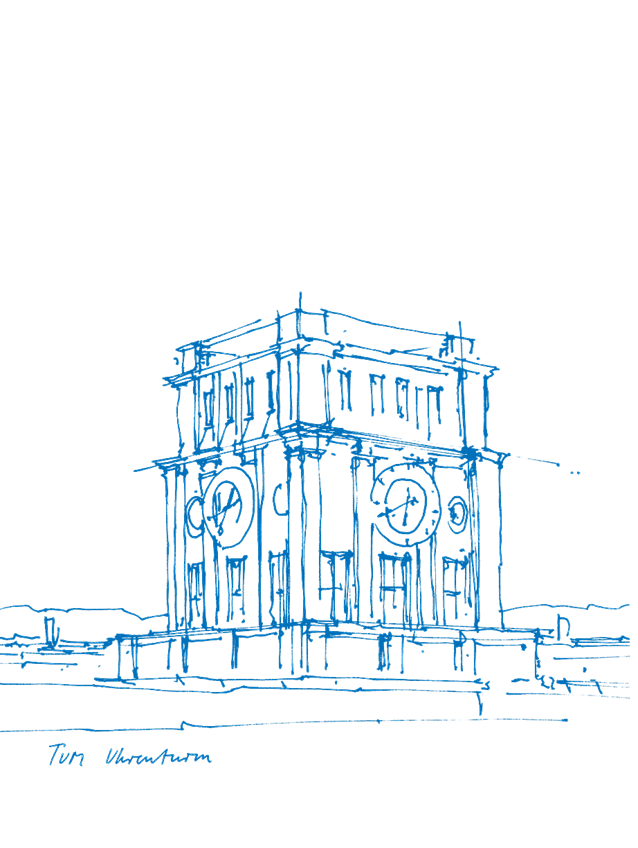
\includegraphics{./Ressources/Presentation/Images/TUM_Uhrenturm.png}%
    \end{textblock*}%
}

\newcommand{\PraesentationStartseiteUhrenturm}{%
    \setbeamertemplate{title page}{%
        \PraesentationSeitenkopfInhalt{./Ressources/_Images/Universitaet_Logo_RGB.pdf}%
        \PraesentationBildUhrenturm%
        \PraesentationTitelseiteInhalt%
    }%
}

\newcommand{\PraesentationStartseiteFlaggen}{%
    \setbeamertemplate{title page}{%
        \begin{textblock*}{\paperwidth}[0,1](-\PraesentationSeitenrand,\paperheight-\PraesentationSeitenrand)%
            
\includegraphics[min width=\paperwidth,max width=\paperheight,min totalsize={\paperwidth}{\paperheight},keepaspectratio,center]{./Ressources/Presentation/Images/Universitaet_Flaggen.jpg}%
        \end{textblock*}%
        \PraesentationSeitenkopfInhalt{./Ressources/_Images/Universitaet_Logo_weiss.pdf}%
        \PraesentationTitelseiteInhalt%
    }%
}

\newcommand{\PraesentationStartseiteLeer}{%
    \setbeamertemplate{title page}{%
        \PraesentationSeitenkopfInhalt{./Ressources/_Images/Universitaet_Logo_weiss.pdf}%
        \PraesentationTitelseiteInhalt%
    }%
}


\newcommand{\PraesentationMasterStandard}{%
    \PraesentationFarbschemaStandard%
    \PraesentationStartseiteUhrenturm%
    \setbeamertemplate{headline}{%
        \PraesentationSeitenkopfInhalt{./Ressources/_Images/Universitaet_Logo_RGB.pdf}%
    }%
}

\newcommand{\PraesentationMasterWeissBlau}{%
    \PraesentationFarbschemaWeissBlau%
    \PraesentationStartseiteLeer%
    \setbeamertemplate{headline}{%
        \PraesentationSeitenkopfInhalt{./Ressources/_Images/Universitaet_Logo_weiss.pdf}%
    }%
}


\newcommand{\PraesentationMasterKopfzeileDreizeiler}{%
    \PraesentationFarbschemaStandard%
    \setbeamertemplate{title page}{%
        \begin{textblock*}{\paperwidth}[0,0](0cm, -7.8mm)%
            \color{TUMBlau}\PraesentationSchriftgroesseDreizeiler\selectfont%
            \LehrstuhlName\\%
            \FakultaetName\\%
            \UniversitaetName\vskip0pt%
            \normalcolor\normalsize\selectfont%
        \end{textblock*}%
        \PraesentationSeitenkopfInhalt{./Ressources/_Images/Universitaet_Logo_RGB.pdf}%
        \PraesentationBildUhrenturm%
        \PraesentationTitelseiteInhalt%
    }%
    \setbeamertemplate{headline}{%
        \begin{textblock*}{\paperwidth}[0,0](0cm, 0cm)%
            \begin{minipage}[t][2cm][t]{\paperwidth}%
                \color{TUMBlau}\PraesentationSchriftgroesseDreizeiler\selectfont%
                \LehrstuhlName\\[1.38mm]%
                \FakultaetName\\[1.44mm]%
                \UniversitaetName\vskip0pt%
                \normalcolor\normalsize\selectfont%
            \end{minipage}%
        \end{textblock*}%
        \PraesentationSeitenkopfInhalt{./Ressources/_Images/Universitaet_Logo_RGB.pdf}%
    }%
}

\newcommand{\PraesentationMasterWeissSchwarz}{%
    \PraesentationFarbschemaWeissSchwarz%
    \setbeamertemplate{title page}{%
        \PraesentationTitelseiteInhalt%
        \PraesentationSeitenkopfInhalt{./Ressources/_Images/Universitaet_Logo_weiss.pdf}%
    }
    \setbeamertemplate{headline}{%
        \PraesentationSeitenkopfInhalt{./Ressources/_Images/Universitaet_Logo_weiss.pdf}%
    }
}

\newcommand{\PraesentationTitelseite}{\frame[plain]{\titlepage}}
\newcommand{\PraesentationUeberschriftZweizeilig}[2]{\frametitle{#1\\[8mm]#2}}

\setbeamersize{
    text margin left=\PraesentationSeitenrand,
    text margin right=\PraesentationSeitenrand
}

\setbeamertemplate{frametitle}{%
    {\rule{0pt}{42mm + \PraesentationPositionKorrekturOben}\PraesentationSchriftgroesseSehrGross\selectfont\insertframetitle\newline\vspace*{-6.7mm}}%
}


% Aufzählungen:
\newcommand{\PraesentationAufzaehlungEbeneEinsSymbol}{\raise2pt\hbox{\donotcoloroutermaths\usebeamercolor{itemize subitem}\PraesentationSchriftgroesseAufzaehlungszeichen$\bullet$}}
\newcommand{\PraesentationAufzaehlungEbeneZweiSymbol}{\raise1.25pt\hbox{\donotcoloroutermaths\usebeamercolor{itemize subitem}$-$}}
\setbeamertemplate{itemize items}[circle]
\setbeamertemplate{itemize subitem}[triangle]
\setbeamercolor{itemize subitem}{fg=black}
\setbeamerfont{itemize/enumerate subbody}{size=\normalsize}
\setbeamertemplate{itemize item}{\PraesentationAufzaehlungEbeneEinsSymbol}
\setbeamertemplate{itemize subitem}{\PraesentationAufzaehlungEbeneZweiSymbol{}}
%\addtolength{\leftmarginii}{16mm-2pt}%

\newenvironment{PraesentationAufzaehlung}
{%
    \vspace{-\baselineskip}%
    \begin{itemize}%
        \setlength{\itemsep}{0pt}%
        \setlength{\parskip}{0pt}%
        \setlength{\parsep}{0pt}%
        \addtolength{\itemindent}{-1ex}%
}{%
    \end{itemize}%
}


\newcommand\Warning{%
	\makebox[1.4em][c]{%
		\makebox[0pt][c]{\raisebox{.1em}{\small!}}%
		\makebox[0pt][c]{\color{TUMOrange}\Large$\bigtriangleup$}}}%

%%%%%%%%%%%%%%%%%%%%%%%%%%%%%%%%%%%%%%%%%%%%%%%%%%%%%%%%%%%%%%%%%%%%%%%%%%%%%%%%
% DOKUMENT
%%%%%%%%%%%%%%%%%%%%%%%%%%%%%%%%%%%%%%%%%%%%%%%%%%%%%%%%%%%%%%%%%%%%%%%%%%%%%%%%


% PDF-Einstellungen:
\hypersetup{
    pdfstartview={Fit},
    pdfproducer={\AllgemeinErsteller},
    pdfcreator={\AllgemeinGestalter}
}

\textblockorigin{\PraesentationSeitenrand}{\PraesentationSeitenrand} % Ursprung für Positionierung

\setbeamerfont{footnote}{size=\PraesentationSchriftgroesseKlein}

\setbeamertemplate{footline}{
    \hbox{%
        \usebeamerfont{footnote}%
        \begin{beamercolorbox}[wd=.9\paperwidth]{}%
            \hspace*{\PraesentationSeitenrand}%
            \PersonTitel{} \PersonVorname~\PersonNachname~(\UniversitaetAbkuerzung) \PraesentationFusszeileZusatz{}%
        \end{beamercolorbox}%
        \begin{beamercolorbox}[wd=.1\paperwidth]{}%
            \insertframenumber{}%
            \raggedleft
            \hspace*{\PraesentationSeitenrand}%
        \end{beamercolorbox}%
        \vspace*{3.25mm}%
    }%
}

\setbeamertemplate{navigation symbols}{}

\begin{document}
\setlength{\baselineskip}{\PraesentationAbstandAbsatz}
\setlength{\parskip}{\baselineskip}
\lstset{language=C++,
		basicstyle=\ttfamily,
		keywordstyle=\color{TUMBlau}\ttfamily,
		stringstyle=\color{TUMOrange}\ttfamily,
		commentstyle=\color{TUMGruen}\ttfamily,
		morecomment=[l][\color{magenta}]{\#},
		aboveskip=0.5\medskipamount,
		belowskip=0.5\medskipamount,
		frame = single,
		numbers=left,
		stepnumber=1,
		escapeinside={(*@}{@*)}
	}
 
%%%%%%%%%%%%%%%%%%%%%%%%%%%%%%%%%%%%%%%%%%%%%%%%%%%%%%%%%%%%%%%%%%%%%%%%%%%%%%%%



%%%%%%%%%%%%%%%%%%%%%%%%%%%%%%%%%%%%%%%%%%%%%%%%%%%%%%%%%%%%%%%%%%%%%%%%%%%%%%%%
% FOLIENSTIL: Standard
% !!!ÄNDERUNG HIER:!!!
\PraesentationMasterStandard
%\PraesentationMasterKopfzeileDreizeiler
%\PraesentationMasterWeissBlau

%\PraesentationStartseiteFlaggen
\PraesentationStartseiteUhrenturm
\PraesentationTitelseite % Fügt die Startseite ein

\begin{frame}
	\frametitle{Overview}
	\vspace{1cm}
	\begin{minipage}[s]{\textwidth}
	\tableofcontents
	\end{minipage}
\end{frame}

\section{The Signorini Problem}
\PraesentationMasterWeissBlau
\begin{frame}[plain, noframenumbering]
	\centering
	\vspace{6cm}
	\huge{\thesection . \secname}
\end{frame}
\PraesentationMasterStandard

\subsection{History and Background}
\begin{frame}
	\frametitle{History and Background}	
	\begin{itemize}
		\item Posed by Antonio Signorini in 1959 in the \textit{Instituto di Alta Matematica}
		\item Find the elastic equilibrium of an elastic body on a frictionless plane
		\item The boundary conditions are ``ambiguous'', i.e. either equality or inequality at any point
		\item Gaetano Fichera solved the problem before Signorini's death, after not finding anything similar in the literature
	\end{itemize}

\begin{itemize}
	\item We will analyze a simpler 1D version of the problem
	\item An elastic beam with a two point contact set on the boundary is subject to an arbitrary force
	\item In the equilibrium configuration, the beam might touch the boundary or not, hence the different boundary conditions
\end{itemize}
\end{frame}

\subsection{The 1D Signorini Problem}
\begin{frame}
	\frametitle{The 1D Signorini Problem}
	\vspace{0.6cm}
	\begin{definition}
		Let $\Omega \coloneqq (-1,1)$,
		
		the normal derivative of $u$ on $\partial\Omega$ be $\partial_nu$, i.e. $\partial_nu(-1) = -u'(-1)$ and $\partial_nu(1) = u'(1)$, 
		
		and $f \in L^2(-1,1)$. The problem is defined as follows:
		\begin{align}
			-u'' + u &= f \quad \textnormal{in} \quad \Omega \label{eq:signorini}\\ 
			\textcolor{TUMBlue}{\partial_n u \geq 0},\quad \textcolor{TUMAccentOrange}{u}\, &\textcolor{TUMAccentOrange}{\geq 0},\textcolor{TUMGray}{\quad u\partial_nu = 0} \quad\textnormal{on}\quad \partial \Omega \label{eq:boundary_signorini}
		\end{align}
		The third boundary condition is the ``ambiguous'' one, as either the beam touches the surface $u(\pm1) = 0$, or it has vanishing derivative on the border $\partial_nu(\pm 1) = 0$.
	\end{definition}
\end{frame}

\subsection{Visualization}
\begin{frame}
	\frametitle{The 1D Signorini Problem}
	\begin{minipage}{0.5\linewidth}
		\vspace{0.6cm}
		Visualization of the problem for a \\right hand side $f = \sin$
	\end{minipage}
	\begin{minipage}{0.5\linewidth}
		\vspace{-3.5cm}
\hspace{8cm}		\begin{tikzpicture}[scale=4.5]
	\draw (-1.25,1) -- (-1,1) -- (-1,0.25);
	\draw (1,0.25) -- (1,1) -- (1.25,1);
	\pattern[pattern=north west lines, pattern color=black] (-1.25,0.25) rectangle (-1,1)
	(1,0.25) rectangle (1.25,1);
	\node[anchor = north] at (-1.125,0.25) {$\vdots$};
	\node[anchor = north] at (1.125,0.25) {$\vdots$};
	
	\draw[thick] plot [smooth] coordinates{(-1,1) (-0.75,0.9451) (-0.5,0.9719) (-0.25,1.0569) (0,1.1764) (0.25,1.3069) (0.5,1.4258) (0.75,1.5116) (1,1.5443)}; 
	
	\draw[->] (-1,2) to 	(-1,	1.5793);
	\draw[->] (-0.75,2) to 	(-0.75,	1.6592);
	\draw[->] (-0.5,2) to 	(-0.5,	1.7603);
	\draw[->] (-0.25,2) to 	(-0.25,	1.8763);
	%\draw[->] (0,2) to 		(0,2);
	\draw[->] (0.25,2) to 	(0.25,	2.1237);
	\draw[->] (0.5,2) to 	(0.5,	2.2397);
	\draw[->] (0.75,2) to 	(0.75,	2.3408);
	\draw[->] (1,2) to 		(1,		2.4207);
	\node at (0,2) {$f$};
	
	\node at (0,1.30) {$u$};
	
	\node[anchor=south] at (-1,1) {$\scriptstyle \substack{\textcolor{TUMAccentOrange}{u(-1) \geq 0} \\ \textcolor{TUMGray}{u (-1) = 0}}$};
	\draw[->] (-1,1) to	(-0.75,	0.85);
	\node[anchor = north] at (-0.75,	0.85) {$\scriptstyle \textcolor{TUMBlue}{\partial_n u(-1) \geq 0}$};
	
	\node[anchor=south] at (1,1.5433) {$\scriptstyle \textcolor{TUMAccentOrange}{u (1) \geq 0}$};
	\draw[->] (1,1.5433) to	(1.25,	1.5433);
	\node[anchor = west] at (1.25,	1.5433) {$\scriptstyle \substack{\textcolor{TUMBlue}{\partial_n u(1) \geq 0} \\ \textcolor{TUMGray}{\partial_nu (1) = 0}}$};
	
	\node[anchor = north] at (0, 0)   {\scriptsize 0};
	\node[anchor = north] at (1, 0)   {\scriptsize 1};
	\node[anchor = north] at (-1, 0)   {\scriptsize -1};
	\node[anchor = east] at (-1.5, 1)   {\scriptsize 0};
	
	\draw[<->] (-1, 0) to (1, 0);
	\draw[<->] (-1.5, 0) to (-1.5, 1);
\end{tikzpicture}	
\end{minipage}
\end{frame}

\section{Solvability}
\PraesentationMasterWeissBlau
\begin{frame}[plain, noframenumbering]
	\centering
	\vspace{6cm}
	\huge{\thesection . \secname}
\end{frame}
\PraesentationMasterStandard
\subsection{Sobolev Spaces}
\begin{frame}
	\frametitle{Solvability - Sobolev Spaces}
	\begin{itemize}
		\item In order to prove the unique solvability of the problem, the above formulation is not adequate
		\item It is only possible to prove this for the weak formulation
		\item We introduce the Sobolev Spaces and some of their important properties, such as the Sobolev Embedding:
	\end{itemize}

\begin{lemma}
	For every $u \in H^k(a,b)$ there exists a $v \in C^{k-1}(a,b)$, such that $u = [v \vert_{(a,b)}]$, i.e.:
	\begin{equation}
		H^k(a,b) \hookrightarrow C^{k-1}(a,b)
	\end{equation}
\end{lemma}

\end{frame}

\subsection{Weak Formulation as a Variational Inequality}
\begin{frame}
\frametitle{Solvability - Weak Formulation I}
\begin{itemize}
	\item Weak formulation means the admissible space of solutions is a superset, and if the solution is in the original set,\\ then it is the classical solution
	\item It is helpful that the superset is a convex subspace of a Banach Space
	\item The most direct weak formulation is as a variational inequality, which follows by integrating by parts:
\end{itemize}
\begin{theorem} 
	Let $K \coloneqq \{ v\in H^1(\Omega) \,|\, v(-1) \geq 0, v(1) \geq 0 \}$. A solution to the following solves the Signorini Problem weakly:
	\begin{equation}
		u \in K,\quad \int_{-1}^1 u'(v'-u') + u(v-u) - f(v-u) \dif x \geq 0 \quad \forall v \in K \label{eq:variational_inequality}
	\end{equation}
	Or, equivalently:
	\begin{equation}
		u \in K,\quad (u,v-u)_{H^1(\Omega)} \geq (f,v-u)_{L^2(\Omega)} \quad \forall v \in K
	\end{equation}
\end{theorem}
\end{frame}

\subsection{Weak Formulation as a Minimization Problem}
\begin{frame}
	\frametitle{Solvability - Weak Formulation II}
	\begin{itemize}
		\item Although we will use similar variational inequalities throughout, it is still not obvious how the solvability can be proved
		\item For that we will reformulate it as a minimization problem, which is equivalent to the variational inequality:
	\end{itemize}

\begin{theorem}
	A solution of the following minimization problem solves the Signorini Problem weakly:
	\begin{equation}
		\min_{\substack{v \in H^1(\Omega) \\ v(-1) \geq 0,\, v(1) \geq 0}} F(v) = \min_{\substack{v \in H^1(\Omega) \\ v(-1) \geq 0,\, v(1) \geq 0}} \int_{-1}^1{\frac{1}{2} (v')^2 + \frac{1}{2} v^2 - fv \dif x} 
	\end{equation}
\end{theorem}

\begin{itemize}
	\item The existence of the solution was proved by the Direct Method of the Calculus of Variations, by showing that $F$ is bounded from below, and $K$ is convex
	\item The uniqueness of the solution follows by the convexness of $F$
	\item We actually prove this for a \textbf{more general set of boundary conditions}
\end{itemize}
\end{frame}

\subsection{$H^2$-regularity of the Solution}
\begin{frame}
	\frametitle{$H^2$-regularity of the Solution}
	\begin{itemize}
		\item We show the following, without further assumptions:
	\end{itemize}
\begin{theorem} 
	Let $u \in H^1(\Omega)$ be a weak solution to the Signorini Problem. Then the following holds for $C \in \mathbb{R}_{>0}:$
	\begin{align}
		u &\in H^2(\Omega) \\
		\norm{u}_{H^2(\Omega)} &\leq C\norm{f}_{L^2(\Omega)}  
	\end{align}
\end{theorem}
\begin{itemize}
	\item This result will be crucial for proving each of the error estimates for the discrete solution
	\item We will realize later in the paper that if $f$ has more regularity, so does $u$
\end{itemize}
\end{frame}

\section{Discretization}
\PraesentationMasterWeissBlau
\begin{frame}[plain, noframenumbering]
	\centering
	\vspace{6cm}
	\huge{\thesection . \secname}
\end{frame}
\PraesentationMasterStandard
\begin{frame}
	\frametitle{Discretization}
	\begin{itemize}
		\item We will approximate solutions by solving the problem in a finite-dimensional subspace
		\item This will be the finite element function space $V_h$ with a uniform mesh width $h$, defined as follows:
	\end{itemize}
\vspace{0.3cm}
\begin{definition}
	\vspace{-0.9cm}
\begin{align}
	V_h \coloneqq \{&z \in C([-1,1]) \, | \, \\ 
	&z \,\, \text{piecewise affine subordinate to a partition}\quad \mathmbox{-1}=x_0<x_1<\dots<x_N = 1 \} \nonumber
\end{align} 
\end{definition}
\vspace{-1cm}
\begin{itemize}
	\item With this, we may define the discrete Signorini Problem:
\end{itemize}
\vspace{0.3cm}
\begin{definition} 
		\vspace{-0.5cm}
	\begin{equation} \label{eq:discrete_minimization}
		\min_{\substack{v_h \in V_h \\ v_h(-1) \geq 0,\, v_h(1) \geq 0}} F(v_h) = \min_{\substack{v_h \in V_h \\ v_h(-1) \geq 0,\, v_h(1) \geq 0}} \int_{-1}^1{\frac{1}{2} (v_h')^2 + \frac{1}{2} v_h^2 - fv_h \dif x} 
	\end{equation}
	Or, equivalently:
	\begin{equation}\label{eq:discrete_variational_inequality}
		u_h \in V_h \cap K,\quad (u_h, v_h-u_h)_{H^1(\Omega)} \geq (f, v_h - u_h)_{L^2(\Omega)} \quad \forall v_h \in V_h \cap K
	\end{equation}
	
\end{definition}
\end{frame}

\begin{frame}
	\frametitle{Discretization - Matrix Form}
	\begin{itemize}
		\item Define for a basis $\{\varphi_i\}$ of $V_h$ the coefficient vector $\mathbf{v}$ for $v_h \in V_h$ as $	v_h(x) = \sum_{i=0}^{N} \mathbf{v}_i \varphi_i^h(x)$
		\item With this representation, the discrete problem can be more clearly written as follows:
	\end{itemize}
		\begin{equation} \label{eq:matrix_formulation}
	\min_{\substack{\mathbf{v} \in \mathbb{R}^{(N+1)}\\ \mathbf{v}_{0} \geq 0,\, \mathbf{v}_N \geq 0}} \frac{1}{2} \mathbf{v}^T (B_1 + B_2) \mathbf{v} - \mathbf{f}^T  \mathbf{v}
\end{equation}
\vspace{-0.8cm}
\begin{itemize}
	\item We call $B_1$ the \emph{mass matrix} and $B_2$ the \emph{stiffness matrix}. $B_1$, $B_2$ and $\mathbf{f} \in \mathbb{R}^{(N+1)}$ are defined as follows:
\end{itemize}
\vspace{-0.5cm}
\begin{align*}
	B_1 \coloneqq 			h	\begin{pmatrix}
		1/3& 1/6 & & & & & \\
		1/6& 2/3& 1/6 & & & & \\
		& 1/6& 2/3& 1/6 & & & \\
		& & & \ddots & & & \\
		& & & 1/6& 2/3& 1/6 & \\
		& & & & 1/6& 2/3& 1/6 \\
		& & & & & 1/6& 1/3
	\end{pmatrix}, \,
	B_2 \coloneqq \frac{1}{h} 			\begin{pmatrix}
		1& -1 & & & & & \\
		-1& 2& -1 & & & & \\
		& -1& 2& -1 & & & \\
		& & & \ddots & & & \\
		& & & -1& 2& -1 & \\
		& & & & -1& 2& -1 \\
		& & & & & -1& 1
	\end{pmatrix}, \,
	\,
	\mathbf{f}_i \coloneqq \phantom{h} \left(\int_{-1}^1 f\varphi_i^h\dif x\right)
\end{align*}
\end{frame}


\section{Error Estimates}
\PraesentationMasterWeissBlau
\begin{frame}[plain, noframenumbering]
	\centering
	\vspace{6cm}
	\huge{\thesection . \secname}
\end{frame}
\PraesentationMasterStandard
\begin{frame}
	\frametitle{Overview}
	\begin{itemize}
		\item We will derive optimal-order error estimates in the $L^{\infty}$, $H^1$ and $H^2$ norms
		\item Optimal in the sense that they are of the same order as the interpolation error for the same equidistant nodes
		\item In this section, let $u \in H^2(\Omega)$ be the unique solution of the Signorini Problem for a fixed $f \in L^2(\Omega)$, $u_h \in V_h$ be the discrete solution for the same $f$
		\item All constants mentioned therefore depend on the choice of $f$
		\item The results we will derive are the following:
	\end{itemize}
	\begin{theorem}
		There exist $C \in \mathbb{R}_{>0}$ such that the following holds:
		\begin{equation}
			\norm{u-u_h}_{L^\infty(\Omega)} \leq C h^{\sfrac{3}{2}}, \quad \norm{u-u_h}_{H^1(\Omega)} \leq C h, \quad 	\norm{u-u_h}_{L^2(\Omega)} \leq Ch^2
		\end{equation}
	\end{theorem}
\end{frame}

\subsection{The Ritz Projection - $L^\infty$ and $H^1$ Errors} 
\begin{frame}
	\frametitle{The Ritz Projection}
	\begin{itemize}
		\item The Ritz Projection $R_h(u)$ is the orthogonal projection from $H^1(\Omega)$ into its subspace $V_h$
		\item Because of orthogonality, it is the solution to the following minimization problem:
	\end{itemize}
	\begin{equation}
		R_h(u) = \argmin_{\substack{v_h \in V_h}} \norm{v_h - u}_{H_1}
	\end{equation}
\vspace{-0.5cm}
\begin{itemize}
	\item The Ritz Projection can also be expressed as the solution $\tilde{u}_h$ to the following (discrete) variational inequality:
\end{itemize}
\begin{equation}\label{eq:ritz_variational}
	(\tilde{u}_h, v_h-\tilde{u}_h)_{H^1(\Omega)} \geq (f, v_h-\tilde{u}_h)_{L^2(\Omega)} \quad \forall v_h \in \tilde{K}_h
\end{equation}
\vspace{-1cm}
\begin{itemize}
	\item where $\tilde{K}_h$ is defined as follows:
\end{itemize}
\vspace{-1cm}
\begin{align*}
	\tilde{K}_h \coloneqq \{v_h \in V_h \,|\,  v_h(1) &\geq (R_h(u) - u)(1) \quad \text{and} \\
	v_h(-1) &\geq (R_h(u) - u)(-1)\}
\end{align*}
\end{frame}

\begin{frame}
	\frametitle{The Ritz Projection - Supercloseness}
	\begin{itemize}
		\item The main result about the Ritz Projection is the following ``supercloseness'' result:
	\end{itemize}
	\begin{equation}\label{eq:supercloseness}
	\norm{u_h - R_h(u)}_{H^1(\Omega)} \leq \frac{7}{3} \max \left(\abs{(u-R_h(u))(-1)}, \abs{(u-R_h(u))(1)}\right) \leq \norm{u-R_h(u)}_{L^{\infty}(\Omega)}
\end{equation}
\vspace{-1cm}
	\begin{itemize}
		\item The discrete solution and the Ritz Projection are ``superclose'' in the $H^1$ and $L^\infty$ norms, i.e. their error order is at least as good as the total error
		\item Using this, known results about the error between the solution and the Ritz Projection, we may derive the total error in the $H^1$ and $L^\infty$ norms by the triangle inequality
		\item Here the $H^2$ regularity is crucial, since the errors of the Ritz Projection use interpolation, which requires regularity of the higher (weak) derivatives
	\end{itemize}
\end{frame}

\subsection{Dual Problems - The $L^2$ Error} 
\begin{frame}
	\frametitle{The Dual Problems}
	\vspace{1cm}
	\begin{definition}
		Firstly, define the following sets of functions fulfilling boundary conditions:
		\begin{align*}
			L \coloneqq \left\{ v \in H^1(\Omega) \,|\, v(\pm 1) \geq 0 \,\,\text{if}\,\, u(\pm 1) = 0 \right\} , \quad
			\tilde{L} \coloneqq \left\{ v \in H^1(\Omega) \,|\, v(\pm 1) \geq 0 \,\,\text{if}\,\, u_h(\pm 1) = 0 \right\}
		\end{align*} 
		Then we define the dual problems as follows:
		\begin{align} 
			z \in L,\quad (z,v-z)_{H^1(\Omega)} \geq (-\max(0,u-u_h),v-z)_{L^2(\Omega)} \quad \forall v \in L \label{eq:dual_variational_inequality} \\
			z \in \tilde{L},\quad (z,v-z)_{H^1(\Omega)} \geq (-\min(0,u_h-u),v-z)_{L^2(\Omega)} \quad \forall v \in \tilde{L}
		\end{align}
	\end{definition}
\vspace{-0.5cm}
\begin{itemize}
	\item We will only analyze the dual problem for the positive component here, since the other one is analogous
	\item Because we generalized the solvability proof of the Signorini Problem, these variational inequalities are also uniquely solvable 
\end{itemize}
\end{frame}

\begin{frame}
	\frametitle{Proof of the $L^2$ Error}
	\begin{itemize}
		\item As already hinted, we split the error into the positive and negative components of the solution
		\item The key inequality to derive is the following (let $z$ be the solution to the positive dual problem):
	\end{itemize}
\begin{equation}
			\norm{\max(0,u-u_h)}_{L^2(\Omega)}^2 \leq (z-I_h(z), u_h - u)_{H^1(\Omega)} \label{eq:scalar_producx_ineq_L2}
\end{equation}
\vspace{-1cm}
\begin{itemize}
	\item Its proof is not trivial, and follows from observations about the solution to the dual problem, Stampacchia's Lemma and the Sobolev Embedding to get inequalities everywhere and not only a.e.
	\item With this inequality, Cauchy-Schwarz, the $H^1$ error result, known results about interpolation error and, again, $H^2$-regularity, the result follows
\end{itemize}
\end{frame}

\section{Numerical Tests}
\PraesentationMasterWeissBlau
\begin{frame}[plain, noframenumbering]
	\centering
	\vspace{6cm}
	\huge{\thesection . \secname}
\end{frame}
\PraesentationMasterStandard

\subsection{Methods}
\begin{frame}
	\frametitle{Methods}
	\begin{itemize}
		\item To calculate the $\mathbf{f}$ vector:
	\end{itemize}
	\begin{equation}
		\mathbf{f}_i = \int_{-1}^1 f\varphi_i^h\dif x = \int_{\max\{-1, x_{i-1}\}}^{\min\{1, x_{i+1}\}} f\varphi_i^h\dif x
	\end{equation} 
\vspace{-1cm}
	\begin{itemize}
		\item To compare a discrete solution to an exact one:
	\end{itemize}
	\begin{align}
		\norm{u-u_h}_{L^\infty(\Omega)} &\approx \max \left\{\abs{u(x) - u_h(x)} \,|\, x \in \{-1 = x_0,\dots, x_n = 1, x_{i+1} - x_i = \sfrac{h}{1000}\} \right\} \\
		\norm{u-u_h}_{L^2(\Omega)} &= \sqrt{\sum_{i=0}^{N-1} \norm{u-u_h}_{L^2(x_i, x_{i+1})}^2 } \\
		\norm{u-u_h}_{H^1(\Omega)} &= \sqrt{\sum_{i=0}^{N-1} \norm{u-u_h}_{L^2(x_i, x_{i+1})}^2 + \sum_{i=0}^{N-1} \norm{u'-u_h'}_{L^2(x_i, x_{i+1})}^2} 
	\end{align}
\end{frame}	
	
\begin{frame}
	\frametitle{Methods}
	\begin{itemize}
		\item To compare a discrete solution to a finer discrete one, the reference solution,
		\item Denote the reference solution vector as $\mathbf{v}^{\tilde{h}}$ and the interpolation of a lower dimensional one into $V_{\tilde{h}}$ as $\tilde{\mathbf{v}}^h$, then the norms can be exactly calculated as follows:
	\end{itemize}
\vspace{-0.7cm}
\begin{align}
	\norm{u_{\tilde{h}} - u_h}_{L^\infty(\Omega)} &= \max_{i \in \{0,\dots,\mathrm{dim} \, V_{\tilde{h}}\}} \abs{\mathbf{v}^{\tilde{h}}_i - \tilde{\mathbf{v}}^h_i} \\
	\norm{u_{\tilde{h}} - u_h}_{L^2(\Omega)} &=  \sqrt{(\mathbf{v}^{\tilde{h}} - \tilde{\mathbf{v}}^h)^T B_1 (\mathbf{v}^{\tilde{h}} - \tilde{\mathbf{v}}^h)}\\
	\norm{u_{\tilde{h}} - u_h}_{H^1(\Omega)} &= \sqrt{(\mathbf{v}^{\tilde{h}} - \tilde{\mathbf{v}}^h)^T (B_1+B_2) (\mathbf{v}^{\tilde{h}} - \tilde{\mathbf{v}}^h)}
\end{align}
\vspace{-1cm}
\begin{itemize}
	\item Finally, to check the convergence orders, we use the Experimental Orders of Convergence (EOCs):
\end{itemize}
\begin{equation}
	(\mathrm{EOC})_{h_k,\,\norm{\cdot}_*} \coloneqq \frac{\log \lVert u-u_{h_k}\rVert_* - \lVert\log u-u_{h_{k-1}}\rVert_* }{\log h_k - \log h_{k-1}}
\end{equation}
\end{frame}

\subsection{Results}
\begin{frame}[c]
	\centering
	\frametitle{Results for $f = \sin$}
		\begin{tabular}{c@{\hskip -1em}c}
			% This file was created by matlab2tikz.
%
%The latest updates can be retrieved from
%  http://www.mathworks.com/matlabcentral/fileexchange/22022-matlab2tikz-matlab2tikz
%where you can also make suggestions and rate matlab2tikz.
%
%
\begin{tikzpicture}[thick,scale=0.6, every node/.style={transform shape}]
\begin{axis}[%
width=4.521in,
height=3.566in,
at={(0.758in,0.481in)},
scale only axis,
xmin=-1,
xmax=1,
ymin=-1,
ymax=1,
axis background/.style={fill=white},
legend style={at={(0.03,0.97)}, anchor=north west, legend cell align=left, align=left, draw=white!15!black}
]
\addplot [color=TUMBlue]
table[row sep=crcr]{%
	-1	-0.841470984807897\\
	-0.9375	-0.806081108260693\\
	-0.875	-0.767543502236027\\
	-0.8125	-0.726008655260713\\
	-0.75	-0.681638760023334\\
	-0.6875	-0.634607080015269\\
	-0.625	-0.585097272940462\\
	-0.5625	-0.53330267353602\\
	-0.5	-0.479425538604203\\
	-0.4375	-0.423676257203938\\
	-0.375	-0.366272529086048\\
	-0.3125	-0.307438514580381\\
	-0.25	-0.247403959254523\\
	-0.1875	-0.18640329676227\\
	-0.125	-0.124674733385228\\
	-0.0625	-0.0624593178423802\\
	0	0\\
	0.0625	0.0624593178423802\\
	0.125	0.124674733385228\\
	0.1875	0.18640329676227\\
	0.25	0.247403959254523\\
	0.3125	0.307438514580381\\
	0.375	0.366272529086048\\
	0.4375	0.423676257203938\\
	0.5	0.479425538604203\\
	0.5625	0.53330267353602\\
	0.625	0.585097272940462\\
	0.6875	0.634607080015269\\
	0.75	0.681638760023334\\
	0.8125	0.726008655260713\\
	0.875	0.767543502236027\\
	0.9375	0.806081108260693\\
	1	0.841470984807897\\
};
\addlegendentry{$\sin(x)$}
\addplot [color=TUMAccentOrange]
table[row sep=crcr]{%
	-1	5.55111512312578e-17\\
	-0.9375	-0.0113404370605935\\
	-0.875	-0.0195764326628391\\
	-0.8125	-0.0248907066684464\\
	-0.75	-0.0274662702214526\\
	-0.6875	-0.0274865073030289\\
	-0.625	-0.0251352144978297\\
	-0.5625	-0.0205966017702051\\
	-0.5	-0.0140552570547911\\
	-0.4375	-0.00569607747220785\\
	-0.375	0.00429583001371972\\
	-0.3125	0.0157352756761656\\
	-0.25	0.0284371390187464\\
	-0.1875	0.0422165428568202\\
	-0.125	0.0568890466623689\\
	-0.0625	0.0722708563519541\\
	0	0.0881790477039399\\
	0.0625	0.104431800601077\\
	0.125	0.120848641307843\\
	0.1875	0.137250690008792\\
	0.25	0.153460910854752\\
	0.3125	0.169304361787987\\
	0.375	0.184608441445637\\
	0.4375	0.199203130472638\\
	0.5	0.212921224611061\\
	0.5625	0.225598556972163\\
	0.625	0.237074206940393\\
	0.6875	0.247190693204885\\
	0.75	0.255794148463479\\
	0.8125	0.262734473396742\\
	0.875	0.267865467564559\\
	0.9375	0.271044934935267\\
	1	0.272134761816798\\
};
\addlegendentry{$u(x)$}
\addplot [color=TUMAccentGreen]
table[row sep=crcr]{%
	-1	2.71500529374605e-18\\
	-0.9375	0.00548243954380626\\
	-0.875	0.0109648790876125\\
	-0.8125	0.0164473186314188\\
	-0.75	0.021929758175225\\
	-0.6875	0.0274121977190313\\
	-0.625	0.0328946372628375\\
	-0.5625	0.0383770768066438\\
	-0.5	0.04385951635045\\
	-0.4375	0.0493419558942563\\
	-0.375	0.0548243954380625\\
	-0.3125	0.0603068349818688\\
	-0.25	0.065789274525675\\
	-0.1875	0.0712717140694813\\
	-0.125	0.0767541536132875\\
	-0.0625	0.0822365931570938\\
	0	0.0877190327009\\
	0.0625	0.0997803996972738\\
	0.125	0.111841766693648\\
	0.1875	0.123903133690021\\
	0.25	0.135964500686395\\
	0.3125	0.148025867682769\\
	0.375	0.160087234679143\\
	0.4375	0.172148601675516\\
	0.5	0.18420996867189\\
	0.5625	0.196271335668264\\
	0.625	0.208332702664638\\
	0.6875	0.220394069661011\\
	0.75	0.232455436657385\\
	0.8125	0.244516803653759\\
	0.875	0.256578170650133\\
	0.9375	0.268639537646506\\
	1	0.28070090464288\\
};
\addlegendentry{$u_h(x)$}
\end{axis}
\begin{axis}[%
width=5.833in,
height=4.375in,
at={(0in,0in)},
scale only axis,
xmin=0,
xmax=1,
ymin=0,
ymax=1,
axis line style={draw=none},
ticks=none,
axis x line*=bottom,
axis y line*=left
]
\end{axis}
\end{tikzpicture}% & % This file was created by matlab2tikz.
%
%The latest updates can be retrieved from
%  http://www.mathworks.com/matlabcentral/fileexchange/22022-matlab2tikz-matlab2tikz
%where you can also make suggestions and rate matlab2tikz.
%
%
\begin{tikzpicture}[thick,scale=0.6, every node/.style={transform shape}]

\begin{axis}[%
width=4.521in,
height=3.566in,
at={(0.758in,0.481in)},
scale only axis,
xmin=-1,
xmax=1,
ymin=-0.3,
ymax=0.3,
axis background/.style={fill=white},
legend style={at={(0.03,0.97)}, anchor=north west, legend cell align=left, align=left, draw=white!15!black}
]
\addplot [color=TUMBlue]
  table[row sep=crcr]{%
-1	-0.20561464735502\\
-0.99609375	-0.202339058170793\\
-0.9921875	-0.199074875884619\\
-0.98828125	-0.195822100591215\\
-0.984375	-0.192580732431921\\
-0.98046875	-0.189350771593396\\
-0.9765625	-0.186132218307407\\
-0.97265625	-0.182925072849613\\
-0.96875	-0.179729335539079\\
-0.96484375	-0.176545006737527\\
-0.9609375	-0.173372086848374\\
-0.95703125	-0.170210576316308\\
-0.953125	-0.167060475626243\\
-0.94921875	-0.163921785302819\\
-0.9453125	-0.160794505909521\\
-0.94140625	-0.157678638048097\\
-0.9375	-0.154574182357536\\
-0.93359375	-0.151481139513706\\
-0.9296875	-0.148399510228458\\
-0.92578125	-0.145329295248871\\
-0.921875	-0.142270495356499\\
-0.91796875	-0.139223111366917\\
-0.9140625	-0.13618714412867\\
-0.91015625	-0.133162594522759\\
-0.90625	-0.130149463461933\\
-0.90234375	-0.127147751889908\\
-0.8984375	-0.124157460780708\\
-0.89453125	-0.121178591138019\\
-0.890625	-0.118211143994301\\
-0.88671875	-0.115255120410367\\
-0.8828125	-0.11231052147447\\
-0.87890625	-0.109377348301763\\
-0.875	-0.106455602033478\\
-0.87109375	-0.103545283836382\\
-0.8671875	-0.100646394901915\\
-0.86328125	-0.0977589364457998\\
-0.859375	-0.0948829097070814\\
-0.85546875	-0.0920183159475272\\
-0.8515625	-0.0891651564510596\\
-0.84765625	-0.0863234325231446\\
-0.84375	-0.0834931454896974\\
-0.83984375	-0.080674296697083\\
-0.8359375	-0.0778668875108224\\
-0.83203125	-0.075070919315408\\
-0.828125	-0.0722863935133802\\
-0.82421875	-0.0695133115247728\\
-0.8203125	-0.0667516747864596\\
-0.81640625	-0.0640014847514578\\
-0.8125	-0.0612627428884025\\
-0.80859375	-0.0585354506807789\\
-0.8046875	-0.0558196096263117\\
-0.80078125	-0.0531152212364532\\
-0.796875	-0.0504222870355733\\
-0.79296875	-0.0477408085603344\\
-0.7890625	-0.0450707873593643\\
-0.78515625	-0.0424122249921908\\
-0.78125	-0.0397651230289426\\
-0.77734375	-0.0371294830495827\\
-0.7734375	-0.0345053066433678\\
-0.76953125	-0.0318925954081806\\
-0.765625	-0.0292913509499471\\
-0.76171875	-0.0267015748819546\\
-0.7578125	-0.0241232688244679\\
-0.75390625	-0.0215564344037205\\
-0.75	-0.0190010732519141\\
-0.74609375	-0.0164571870058694\\
-0.7421875	-0.0139247773071247\\
-0.73828125	-0.0114038458009702\\
-0.734375	-0.00889439413590765\\
-0.73046875	-0.00639642396303941\\
-0.7265625	-0.00390993693572739\\
-0.72265625	-0.00143493470862666\\
-0.71875	0.00102858106262715\\
-0.71484375	0.00348060872192946\\
-0.7109375	0.00592114661377252\\
-0.70703125	0.00835019308298968\\
-0.703125	0.0107677464761764\\
-0.69921875	0.0131738051416193\\
-0.6953125	0.0155683674303475\\
-0.69140625	0.01795143169619\\
-0.6875	0.0203229962968265\\
-0.68359375	0.0226830595940157\\
-0.6796875	0.0250316199541771\\
-0.67578125	0.0273686757492015\\
-0.671875	0.0296942253566499\\
-0.66796875	0.032008267160478\\
-0.6640625	0.0343107995516192\\
-0.66015625	0.0366018209283965\\
-0.65625	0.0388813296971477\\
-0.65234375	0.0411493242727232\\
-0.6484375	0.0434058030790681\\
-0.64453125	0.0456507645495918\\
-0.640625	0.0478842071279928\\
-0.63671875	0.0501061292684\\
-0.6328125	0.0523165294362258\\
-0.62890625	0.0545154061084787\\
-0.625	0.0567027577744454\\
-0.62109375	0.058878582935975\\
-0.6171875	0.0610428801081753\\
-0.61328125	0.0631956478199101\\
-0.609375	0.0653368846141262\\
-0.60546875	0.0674665890486779\\
-0.6015625	0.0695847596964541\\
-0.59765625	0.0716913951461464\\
-0.59375	0.0737864940025901\\
-0.58984375	0.0758700548873747\\
-0.5859375	0.0779420764392285\\
-0.58203125	0.0800025573145291\\
-0.578125	0.0820514961878587\\
-0.57421875	0.084088891752387\\
-0.5703125	0.0861147427203548\\
-0.56640625	0.0881290478236565\\
-0.5625	0.0901318058141882\\
-0.55859375	0.0921230154643808\\
-0.5546875	0.0941026755676333\\
-0.55078125	0.0960707849387887\\
-0.546875	0.0980273424146532\\
-0.54296875	0.0999723468543294\\
-0.5390625	0.1019057971398\\
-0.53515625	0.103827692176274\\
-0.53125	0.105738030892752\\
-0.52734375	0.107636812242319\\
-0.5234375	0.109524035202767\\
-0.51953125	0.111399698776886\\
-0.515625	0.113263801993007\\
-0.51171875	0.115116343905392\\
-0.5078125	0.116957323594626\\
-0.50390625	0.11878674016819\\
-0.5	0.120604592760664\\
-0.49609375	0.12241088053441\\
-0.4921875	0.124205602679822\\
-0.48828125	0.12598875841578\\
-0.484375	0.127760346990087\\
-0.48046875	0.129520367679916\\
-0.4765625	0.131268819792112\\
-0.47265625	0.133005702663745\\
-0.46875	0.134731015662439\\
-0.46484375	0.136444758186791\\
-0.4609375	0.138146929666668\\
-0.45703125	0.139837529563849\\
-0.453125	0.141516557372192\\
-0.44921875	0.143184012618107\\
-0.4453125	0.144839894861043\\
-0.44140625	0.146484203693689\\
-0.4375	0.148116938742476\\
-0.43359375	0.14973809966795\\
-0.4296875	0.151347686165195\\
-0.42578125	0.15294569796405\\
-0.421875	0.154532134829687\\
-0.41796875	0.156106996562876\\
-0.4140625	0.157670283000286\\
-0.41015625	0.15922199401502\\
-0.40625	0.160762129516876\\
-0.40234375	0.162290689452696\\
-0.3984375	0.163807673806737\\
-0.39453125	0.165313082601116\\
-0.390625	0.166806915896004\\
-0.38671875	0.168289173790136\\
-0.3828125	0.16975985642101\\
-0.37890625	0.171218963965345\\
-0.375	0.172666496639437\\
-0.37109375	0.174102454699323\\
-0.3671875	0.175526838441371\\
-0.36328125	0.176939648202378\\
-0.359375	0.17834088436009\\
-0.35546875	0.179730547333406\\
-0.3515625	0.18110863758276\\
-0.34765625	0.182475155610412\\
-0.34375	0.183830101960837\\
-0.33984375	0.18517347722095\\
-0.3359375	0.186505282020491\\
-0.33203125	0.187825517032287\\
-0.328125	0.189134182972623\\
-0.32421875	0.190431280601501\\
-0.3203125	0.191716810722944\\
-0.31640625	0.192990774185333\\
-0.3125	0.194253171881684\\
-0.30859375	0.195504004749949\\
-0.3046875	0.196743273773251\\
-0.30078125	0.19797097998034\\
-0.296875	0.199187124445707\\
-0.29296875	0.200391708289892\\
-0.2890625	0.201584732679926\\
-0.28515625	0.202766198829401\\
-0.28125	0.203936107998871\\
-0.27734375	0.205094461496145\\
-0.2734375	0.206241260676428\\
-0.26953125	0.207376506942744\\
-0.265625	0.208500201746112\\
-0.26171875	0.209612346585843\\
-0.2578125	0.210712943009803\\
-0.25390625	0.211801992614578\\
-0.25	0.212879497045972\\
-0.24609375	0.21394545799895\\
-0.2421875	0.214999877218137\\
-0.23828125	0.216042756497913\\
-0.234375	0.217074097682762\\
-0.23046875	0.218093902667416\\
-0.2265625	0.219102173397228\\
-0.22265625	0.220098911868238\\
-0.21875	0.221084120127564\\
-0.21484375	0.222057800273532\\
-0.2109375	0.223019954455985\\
-0.20703125	0.223970584876415\\
-0.203125	0.22490969378827\\
-0.19921875	0.22583728349715\\
-0.1953125	0.226753356360998\\
-0.19140625	0.22765791479037\\
-0.1875	0.228550961248565\\
-0.18359375	0.229432498251949\\
-0.1796875	0.230302528370068\\
-0.17578125	0.231161054225861\\
-0.171875	0.232008078495966\\
-0.16796875	0.232843603910766\\
-0.1640625	0.233667633254687\\
-0.16015625	0.234480169366361\\
-0.15625	0.235281215138858\\
-0.15234375	0.236070773519824\\
-0.1484375	0.236848847511624\\
-0.14453125	0.237615440171709\\
-0.140625	0.23837055461258\\
-0.13671875	0.23911419400206\\
-0.1328125	0.239846361563551\\
-0.12890625	0.240567060576055\\
-0.125	0.241276294374435\\
-0.12109375	0.241974066349576\\
-0.1171875	0.242660379948546\\
-0.11328125	0.2433352386747\\
-0.109375	0.24399864608799\\
-0.10546875	0.244650605804891\\
-0.1015625	0.245291121498816\\
-0.09765625	0.245920196900066\\
-0.09375	0.246537835796083\\
-0.08984375	0.247144042031515\\
-0.0859375	0.247738819508506\\
-0.08203125	0.248322172186619\\
-0.078125	0.248894104083234\\
-0.07421875	0.249454619273457\\
-0.0703125	0.25000372189033\\
-0.06640625	0.250541416125049\\
-0.0625	0.251067706226966\\
-0.05859375	0.251582596503791\\
-0.0546875	0.252086091321665\\
-0.05078125	0.252578195105329\\
-0.046875	0.253058912338187\\
-0.04296875	0.253528247562514\\
-0.0390625	0.253986205379405\\
-0.03515625	0.254432790449076\\
-0.03125	0.254868007490824\\
-0.02734375	0.255291861283219\\
-0.0234375	0.255704356664157\\
-0.01953125	0.256105498530935\\
-0.015625	0.256495291840473\\
-0.01171875	0.256873741609233\\
-0.0078125	0.25724085291343\\
-0.00390625	0.25759663088914\\
0	0.25794108073222\\
0.00390625	0.258274207698584\\
0.0078125	0.258596017104207\\
0.01171875	0.258906514325133\\
0.015625	0.259205704797687\\
0.01953125	0.259493594018426\\
0.0234375	0.259770187544277\\
0.02734375	0.260035490992589\\
0.03125	0.260289510041172\\
0.03515625	0.260532250428408\\
0.0390625	0.260763717953271\\
0.04296875	0.260983918475365\\
0.046875	0.261192857915049\\
0.05078125	0.261390542253444\\
0.0546875	0.261576977532464\\
0.05859375	0.261752169854859\\
0.0625	0.261916125384364\\
0.06640625	0.26206885034556\\
0.0703125	0.262210351024098\\
0.07421875	0.262340633766552\\
0.078125	0.26245970498065\\
0.08203125	0.262567571135115\\
0.0859375	0.262664238759825\\
0.08984375	0.262749714445775\\
0.09375	0.262824004845108\\
0.09765625	0.262887116671166\\
0.1015625	0.262939056698478\\
0.10546875	0.26297983176277\\
0.109375	0.263009448760965\\
0.11328125	0.263027914651282\\
0.1171875	0.263035236453117\\
0.12109375	0.263031421247124\\
0.125	0.26301647617521\\
0.12890625	0.262990408440501\\
0.1328125	0.262953225307403\\
0.13671875	0.262904934101496\\
0.140625	0.262845542209622\\
0.14453125	0.262775057079821\\
0.1484375	0.262693486221366\\
0.15234375	0.262600837204616\\
0.15625	0.262497117661241\\
0.16015625	0.262382335283888\\
0.1640625	0.262256497826471\\
0.16796875	0.262119613103884\\
0.171875	0.261971688992119\\
0.17578125	0.261812733428236\\
0.1796875	0.261642754410225\\
0.18359375	0.261461759997069\\
0.1875	0.261269758308671\\
0.19140625	0.261066757525811\\
0.1953125	0.260852765890043\\
0.19921875	0.260627791703811\\
0.203125	0.260391843330218\\
0.20703125	0.260144929193046\\
0.2109375	0.259887057776744\\
0.21484375	0.259618237626306\\
0.21875	0.259338477347242\\
0.22265625	0.259047785605503\\
0.2265625	0.258746171127413\\
0.23046875	0.258433642699636\\
0.234375	0.258110209169068\\
0.23828125	0.257775879442761\\
0.2421875	0.25743066248787\\
0.24609375	0.257074567331593\\
0.25	0.256707603061024\\
0.25390625	0.256329778823165\\
0.2578125	0.255941103824696\\
0.26171875	0.255541587332083\\
0.265625	0.255131238671325\\
0.26953125	0.254710067227919\\
0.2734375	0.254278082446795\\
0.27734375	0.253835293832132\\
0.28125	0.253381710947373\\
0.28515625	0.252917343415035\\
0.2890625	0.252442200916597\\
0.29296875	0.251956293192499\\
0.296875	0.251459630041893\\
0.30078125	0.250952221322592\\
0.3046875	0.250434076951052\\
0.30859375	0.249905206901985\\
0.3125	0.249365621208597\\
0.31640625	0.248815329962127\\
0.3203125	0.248254343311999\\
0.32421875	0.247682671465469\\
0.328125	0.247100324687658\\
0.33203125	0.246507313301301\\
0.3359375	0.245903647686745\\
0.33984375	0.245289338281609\\
0.34375	0.244664395580912\\
0.34765625	0.244028830136656\\
0.3515625	0.243382652557898\\
0.35546875	0.242725873510437\\
0.359375	0.242058503716812\\
0.36328125	0.24138055395602\\
0.3671875	0.240692035063439\\
0.37109375	0.239992957930646\\
0.375	0.239283333505263\\
0.37890625	0.238563172790776\\
0.3828125	0.237832486846401\\
0.38671875	0.237091286786843\\
0.390625	0.236339583782303\\
0.39453125	0.235577389058037\\
0.3984375	0.234804713894448\\
0.40234375	0.234021569626691\\
0.40625	0.23322796764468\\
0.41015625	0.23242391939273\\
0.4140625	0.231609436369553\\
0.41796875	0.230784530127863\\
0.421875	0.229949212274406\\
0.42578125	0.229103494469626\\
0.4296875	0.22824738842742\\
0.43359375	0.227380905915197\\
0.4375	0.226504058753349\\
0.44140625	0.2256168588153\\
0.4453125	0.224719318027184\\
0.44921875	0.223811448367663\\
0.453125	0.222893261867718\\
0.45703125	0.221964770610434\\
0.4609375	0.221025986730844\\
0.46484375	0.220076922415558\\
0.46875	0.219117589902766\\
0.47265625	0.218148001481808\\
0.4765625	0.217168169493092\\
0.48046875	0.216178106327781\\
0.484375	0.21517782442762\\
0.48828125	0.214167336284703\\
0.4921875	0.213146654441196\\
0.49609375	0.212115791489133\\
0.5	0.21107476007019\\
0.50390625	0.210023572875407\\
0.5078125	0.208962242645008\\
0.51171875	0.207890782168057\\
0.515625	0.20680920428233\\
0.51953125	0.205717521873979\\
0.5234375	0.204615747877277\\
0.52734375	0.203503895274473\\
0.53125	0.202381977095364\\
0.53515625	0.20125000641719\\
0.5390625	0.200107996364309\\
0.54296875	0.198955960107924\\
0.546875	0.197793910865755\\
0.55078125	0.196621861902017\\
0.5546875	0.195439826526801\\
0.55859375	0.194247818096095\\
0.5625	0.193045850011316\\
0.56640625	0.191833935719188\\
0.5703125	0.190612088711269\\
0.57421875	0.189380322523881\\
0.578125	0.188138650737685\\
0.58203125	0.18688708697745\\
0.5859375	0.185625644911731\\
0.58984375	0.184354338252582\\
0.59375	0.183073180755343\\
0.59765625	0.181782186218186\\
0.6015625	0.180481368481992\\
0.60546875	0.179170741429907\\
0.609375	0.177850318987133\\
0.61328125	0.176520115120553\\
0.6171875	0.175180143838489\\
0.62109375	0.173830419190352\\
0.625	0.172470955266334\\
0.62890625	0.171101766197147\\
0.6328125	0.169722866153585\\
0.63671875	0.168334269346289\\
0.640625	0.166935990025451\\
0.64453125	0.165528042480503\\
0.6484375	0.164110441039618\\
0.65234375	0.162683200069601\\
0.65625	0.161246333975456\\
0.66015625	0.159799857200014\\
0.6640625	0.158343784223732\\
0.66796875	0.156878129564191\\
0.671875	0.155402907775894\\
0.67578125	0.153918133449835\\
0.6796875	0.152423821213219\\
0.68359375	0.150919985729075\\
0.6875	0.149406641695897\\
0.69140625	0.147883803847371\\
0.6953125	0.146351486951907\\
0.69921875	0.144809705812413\\
0.703125	0.143258475265782\\
0.70703125	0.141697810182762\\
0.7109375	0.140127725467252\\
0.71484375	0.138548236056394\\
0.71875	0.136959356919704\\
0.72265625	0.135361103059154\\
0.7265625	0.133753489508493\\
0.73046875	0.132136531332989\\
0.734375	0.130510243629161\\
0.73828125	0.128874641524149\\
0.7421875	0.127229740175537\\
0.74609375	0.125575554770919\\
0.75	0.12391210052759\\
0.75390625	0.122239392691881\\
0.7578125	0.120557446539209\\
0.76171875	0.118866277373257\\
0.765625	0.117165900525933\\
0.76953125	0.115456331356683\\
0.7734375	0.113737585252338\\
0.77734375	0.112009677626531\\
0.78125	0.110272623919442\\
0.78515625	0.108526439597313\\
0.7890625	0.106771140152034\\
0.79296875	0.105006741100752\\
0.796875	0.103233257985551\\
0.80078125	0.101450706372887\\
0.8046875	0.0996591018532769\\
0.80859375	0.0978584600408396\\
0.8125	0.0960487965729584\\
0.81640625	0.094230127109725\\
0.8203125	0.0924024673336277\\
0.82421875	0.0905658329491246\\
0.828125	0.0887202396821039\\
0.83203125	0.086865703279642\\
0.8359375	0.0850022395093788\\
0.83984375	0.0831298641592895\\
0.84375	0.0812485930369888\\
0.84765625	0.0793584419696032\\
0.8515625	0.0774594268030313\\
0.85546875	0.075551563401774\\
0.859375	0.073634867648309\\
0.86328125	0.0717093554426782\\
0.8671875	0.0697750427021333\\
0.87109375	0.0678319453605667\\
0.875	0.0658800793681138\\
0.87890625	0.0639194606907836\\
0.8828125	0.061950105309819\\
0.88671875	0.0599720292213846\\
0.890625	0.057985248436097\\
0.89453125	0.0559897789785424\\
0.8984375	0.0539856368866936\\
0.90234375	0.0519728382117535\\
0.90625	0.0499513990172602\\
0.91015625	0.047921335379101\\
0.9140625	0.0458826633845888\\
0.91796875	0.0438353991323055\\
0.921875	0.0417795587314771\\
0.92578125	0.0397151583015329\\
0.9296875	0.037642213971651\\
0.93359375	0.0355607418802606\\
0.9375	0.0334707581744738\\
0.94140625	0.0313722790098296\\
0.9453125	0.0292653205495412\\
0.94921875	0.0271498989641401\\
0.953125	0.0250260304310075\\
0.95703125	0.0228937311338484\\
0.9609375	0.0207530172621659\\
0.96484375	0.0186039050107922\\
0.96875	0.0164464105794195\\
0.97265625	0.0142805501720318\\
0.9765625	0.0121063399964783\\
0.98046875	0.00992379626393358\\
0.984375	0.00773293518837193\\
0.98828125	0.0055337729860554\\
0.9921875	0.00332632587507931\\
0.99609375	0.00111061007486057\\
};
\addlegendentry{$u'(x)$}

\addplot [color=TUMAccentOrange]
  table[row sep=crcr]{%
-1	-0.110768975308095\\
-0.99609375	-0.110768975308095\\
-0.9921875	-0.110768975308095\\
-0.98828125	-0.110768975308095\\
-0.984375	-0.110768975308095\\
-0.98046875	-0.110768975308095\\
-0.9765625	-0.110768975308095\\
-0.97265625	-0.110768975308095\\
-0.96875	-0.110768975308095\\
-0.96484375	-0.110768975308095\\
-0.9609375	-0.110768975308095\\
-0.95703125	-0.110768975308095\\
-0.953125	-0.110768975308095\\
-0.94921875	-0.110768975308095\\
-0.9453125	-0.110768975308095\\
-0.94140625	-0.110768975308095\\
-0.9375	-0.110768975308095\\
-0.93359375	-0.110768975308095\\
-0.9296875	-0.110768975308095\\
-0.92578125	-0.110768975308095\\
-0.921875	-0.110768975308095\\
-0.91796875	-0.110768975308095\\
-0.9140625	-0.110768975308095\\
-0.91015625	-0.110768975308095\\
-0.90625	-0.110768975308095\\
-0.90234375	-0.110768975308095\\
-0.8984375	-0.110768975308095\\
-0.89453125	-0.110768975308095\\
-0.890625	-0.110768975308095\\
-0.88671875	-0.110768975308095\\
-0.8828125	-0.110768975308095\\
-0.87890625	-0.110768975308095\\
-0.875	-0.110768975308095\\
-0.87109375	-0.110768975308095\\
-0.8671875	-0.110768975308095\\
-0.86328125	-0.110768975308095\\
-0.859375	-0.110768975308095\\
-0.85546875	-0.110768975308095\\
-0.8515625	-0.110768975308095\\
-0.84765625	-0.110768975308095\\
-0.84375	-0.110768975308095\\
-0.83984375	-0.110768975308095\\
-0.8359375	-0.110768975308095\\
-0.83203125	-0.110768975308095\\
-0.828125	-0.110768975308095\\
-0.82421875	-0.110768975308095\\
-0.8203125	-0.110768975308095\\
-0.81640625	-0.110768975308095\\
-0.8125	-0.110768975308095\\
-0.80859375	-0.110768975308095\\
-0.8046875	-0.110768975308095\\
-0.80078125	-0.110768975308095\\
-0.796875	-0.110768975308095\\
-0.79296875	-0.110768975308095\\
-0.7890625	-0.110768975308095\\
-0.78515625	-0.110768975308095\\
-0.78125	-0.110768975308095\\
-0.77734375	-0.110768975308095\\
-0.7734375	-0.110768975308095\\
-0.76953125	-0.110768975308095\\
-0.765625	-0.110768975308095\\
-0.76171875	-0.110768975308095\\
-0.7578125	-0.110768975308095\\
-0.75390625	-0.110768975308095\\
-0.75	0.0535435389637566\\
-0.74609375	0.0535435389637566\\
-0.7421875	0.0535435389637566\\
-0.73828125	0.0535435389637566\\
-0.734375	0.0535435389637566\\
-0.73046875	0.0535435389637566\\
-0.7265625	0.0535435389637566\\
-0.72265625	0.0535435389637566\\
-0.71875	0.0535435389637566\\
-0.71484375	0.0535435389637566\\
-0.7109375	0.0535435389637566\\
-0.70703125	0.0535435389637566\\
-0.703125	0.0535435389637566\\
-0.69921875	0.0535435389637566\\
-0.6953125	0.0535435389637566\\
-0.69140625	0.0535435389637566\\
-0.6875	0.0535435389637566\\
-0.68359375	0.0535435389637566\\
-0.6796875	0.0535435389637566\\
-0.67578125	0.0535435389637566\\
-0.671875	0.0535435389637566\\
-0.66796875	0.0535435389637566\\
-0.6640625	0.0535435389637566\\
-0.66015625	0.0535435389637566\\
-0.65625	0.0535435389637566\\
-0.65234375	0.0535435389637566\\
-0.6484375	0.0535435389637566\\
-0.64453125	0.0535435389637566\\
-0.640625	0.0535435389637566\\
-0.63671875	0.0535435389637566\\
-0.6328125	0.0535435389637566\\
-0.62890625	0.0535435389637566\\
-0.625	0.0535435389637566\\
-0.62109375	0.0535435389637566\\
-0.6171875	0.0535435389637566\\
-0.61328125	0.0535435389637566\\
-0.609375	0.0535435389637566\\
-0.60546875	0.0535435389637566\\
-0.6015625	0.0535435389637566\\
-0.59765625	0.0535435389637566\\
-0.59375	0.0535435389637566\\
-0.58984375	0.0535435389637566\\
-0.5859375	0.0535435389637566\\
-0.58203125	0.0535435389637566\\
-0.578125	0.0535435389637566\\
-0.57421875	0.0535435389637566\\
-0.5703125	0.0535435389637566\\
-0.56640625	0.0535435389637566\\
-0.5625	0.0535435389637566\\
-0.55859375	0.0535435389637566\\
-0.5546875	0.0535435389637566\\
-0.55078125	0.0535435389637566\\
-0.546875	0.0535435389637566\\
-0.54296875	0.0535435389637566\\
-0.5390625	0.0535435389637566\\
-0.53515625	0.0535435389637566\\
-0.53125	0.0535435389637566\\
-0.52734375	0.0535435389637566\\
-0.5234375	0.0535435389637566\\
-0.51953125	0.0535435389637566\\
-0.515625	0.0535435389637566\\
-0.51171875	0.0535435389637566\\
-0.5078125	0.0535435389637566\\
-0.50390625	0.0535435389637566\\
-0.5	0.170417821356017\\
-0.49609375	0.170417821356017\\
-0.4921875	0.170417821356017\\
-0.48828125	0.170417821356017\\
-0.484375	0.170417821356017\\
-0.48046875	0.170417821356017\\
-0.4765625	0.170417821356017\\
-0.47265625	0.170417821356017\\
-0.46875	0.170417821356017\\
-0.46484375	0.170417821356017\\
-0.4609375	0.170417821356017\\
-0.45703125	0.170417821356017\\
-0.453125	0.170417821356017\\
-0.44921875	0.170417821356017\\
-0.4453125	0.170417821356017\\
-0.44140625	0.170417821356017\\
-0.4375	0.170417821356017\\
-0.43359375	0.170417821356017\\
-0.4296875	0.170417821356017\\
-0.42578125	0.170417821356017\\
-0.421875	0.170417821356017\\
-0.41796875	0.170417821356017\\
-0.4140625	0.170417821356017\\
-0.41015625	0.170417821356017\\
-0.40625	0.170417821356017\\
-0.40234375	0.170417821356017\\
-0.3984375	0.170417821356017\\
-0.39453125	0.170417821356017\\
-0.390625	0.170417821356017\\
-0.38671875	0.170417821356017\\
-0.3828125	0.170417821356017\\
-0.37890625	0.170417821356017\\
-0.375	0.170417821356017\\
-0.37109375	0.170417821356017\\
-0.3671875	0.170417821356017\\
-0.36328125	0.170417821356017\\
-0.359375	0.170417821356017\\
-0.35546875	0.170417821356017\\
-0.3515625	0.170417821356017\\
-0.34765625	0.170417821356017\\
-0.34375	0.170417821356017\\
-0.33984375	0.170417821356017\\
-0.3359375	0.170417821356017\\
-0.33203125	0.170417821356017\\
-0.328125	0.170417821356017\\
-0.32421875	0.170417821356017\\
-0.3203125	0.170417821356017\\
-0.31640625	0.170417821356017\\
-0.3125	0.170417821356017\\
-0.30859375	0.170417821356017\\
-0.3046875	0.170417821356017\\
-0.30078125	0.170417821356017\\
-0.296875	0.170417821356017\\
-0.29296875	0.170417821356017\\
-0.2890625	0.170417821356017\\
-0.28515625	0.170417821356017\\
-0.28125	0.170417821356017\\
-0.27734375	0.170417821356017\\
-0.2734375	0.170417821356017\\
-0.26953125	0.170417821356017\\
-0.265625	0.170417821356017\\
-0.26171875	0.170417821356017\\
-0.2578125	0.170417821356017\\
-0.25390625	0.170417821356017\\
-0.25	0.239744012866856\\
-0.24609375	0.239744012866856\\
-0.2421875	0.239744012866856\\
-0.23828125	0.239744012866856\\
-0.234375	0.239744012866856\\
-0.23046875	0.239744012866856\\
-0.2265625	0.239744012866856\\
-0.22265625	0.239744012866856\\
-0.21875	0.239744012866856\\
-0.21484375	0.239744012866856\\
-0.2109375	0.239744012866856\\
-0.20703125	0.239744012866856\\
-0.203125	0.239744012866856\\
-0.19921875	0.239744012866856\\
-0.1953125	0.239744012866856\\
-0.19140625	0.239744012866856\\
-0.1875	0.239744012866856\\
-0.18359375	0.239744012866856\\
-0.1796875	0.239744012866856\\
-0.17578125	0.239744012866856\\
-0.171875	0.239744012866856\\
-0.16796875	0.239744012866856\\
-0.1640625	0.239744012866856\\
-0.16015625	0.239744012866856\\
-0.15625	0.239744012866856\\
-0.15234375	0.239744012866856\\
-0.1484375	0.239744012866856\\
-0.14453125	0.239744012866856\\
-0.140625	0.239744012866856\\
-0.13671875	0.239744012866856\\
-0.1328125	0.239744012866856\\
-0.12890625	0.239744012866856\\
-0.125	0.239744012866856\\
-0.12109375	0.239744012866856\\
-0.1171875	0.239744012866856\\
-0.11328125	0.239744012866856\\
-0.109375	0.239744012866856\\
-0.10546875	0.239744012866856\\
-0.1015625	0.239744012866856\\
-0.09765625	0.239744012866856\\
-0.09375	0.239744012866856\\
-0.08984375	0.239744012866856\\
-0.0859375	0.239744012866856\\
-0.08203125	0.239744012866856\\
-0.078125	0.239744012866856\\
-0.07421875	0.239744012866856\\
-0.0703125	0.239744012866856\\
-0.06640625	0.239744012866856\\
-0.0625	0.239744012866856\\
-0.05859375	0.239744012866856\\
-0.0546875	0.239744012866856\\
-0.05078125	0.239744012866856\\
-0.046875	0.239744012866856\\
-0.04296875	0.239744012866856\\
-0.0390625	0.239744012866856\\
-0.03515625	0.239744012866856\\
-0.03125	0.239744012866856\\
-0.02734375	0.239744012866856\\
-0.0234375	0.239744012866856\\
-0.01953125	0.239744012866856\\
-0.015625	0.239744012866856\\
-0.01171875	0.239744012866856\\
-0.0078125	0.239744012866856\\
-0.00390625	0.239744012866856\\
0	0.262034732732869\\
0.00390625	0.262034732732869\\
0.0078125	0.262034732732869\\
0.01171875	0.262034732732869\\
0.015625	0.262034732732869\\
0.01953125	0.262034732732869\\
0.0234375	0.262034732732869\\
0.02734375	0.262034732732869\\
0.03125	0.262034732732869\\
0.03515625	0.262034732732869\\
0.0390625	0.262034732732869\\
0.04296875	0.262034732732869\\
0.046875	0.262034732732869\\
0.05078125	0.262034732732869\\
0.0546875	0.262034732732869\\
0.05859375	0.262034732732869\\
0.0625	0.262034732732869\\
0.06640625	0.262034732732869\\
0.0703125	0.262034732732869\\
0.07421875	0.262034732732869\\
0.078125	0.262034732732869\\
0.08203125	0.262034732732869\\
0.0859375	0.262034732732869\\
0.08984375	0.262034732732869\\
0.09375	0.262034732732869\\
0.09765625	0.262034732732869\\
0.1015625	0.262034732732869\\
0.10546875	0.262034732732869\\
0.109375	0.262034732732869\\
0.11328125	0.262034732732869\\
0.1171875	0.262034732732869\\
0.12109375	0.262034732732869\\
0.125	0.262034732732869\\
0.12890625	0.262034732732869\\
0.1328125	0.262034732732869\\
0.13671875	0.262034732732869\\
0.140625	0.262034732732869\\
0.14453125	0.262034732732869\\
0.1484375	0.262034732732869\\
0.15234375	0.262034732732869\\
0.15625	0.262034732732869\\
0.16015625	0.262034732732869\\
0.1640625	0.262034732732869\\
0.16796875	0.262034732732869\\
0.171875	0.262034732732869\\
0.17578125	0.262034732732869\\
0.1796875	0.262034732732869\\
0.18359375	0.262034732732869\\
0.1875	0.262034732732869\\
0.19140625	0.262034732732869\\
0.1953125	0.262034732732869\\
0.19921875	0.262034732732869\\
0.203125	0.262034732732869\\
0.20703125	0.262034732732869\\
0.2109375	0.262034732732869\\
0.21484375	0.262034732732869\\
0.21875	0.262034732732869\\
0.22265625	0.262034732732869\\
0.2265625	0.262034732732869\\
0.23046875	0.262034732732869\\
0.234375	0.262034732732869\\
0.23828125	0.262034732732869\\
0.2421875	0.262034732732869\\
0.24609375	0.262034732732869\\
0.25	0.238697815892961\\
0.25390625	0.238697815892961\\
0.2578125	0.238697815892961\\
0.26171875	0.238697815892961\\
0.265625	0.238697815892961\\
0.26953125	0.238697815892961\\
0.2734375	0.238697815892961\\
0.27734375	0.238697815892961\\
0.28125	0.238697815892961\\
0.28515625	0.238697815892961\\
0.2890625	0.238697815892961\\
0.29296875	0.238697815892961\\
0.296875	0.238697815892961\\
0.30078125	0.238697815892961\\
0.3046875	0.238697815892961\\
0.30859375	0.238697815892961\\
0.3125	0.238697815892961\\
0.31640625	0.238697815892961\\
0.3203125	0.238697815892961\\
0.32421875	0.238697815892961\\
0.328125	0.238697815892961\\
0.33203125	0.238697815892961\\
0.3359375	0.238697815892961\\
0.33984375	0.238697815892961\\
0.34375	0.238697815892961\\
0.34765625	0.238697815892961\\
0.3515625	0.238697815892961\\
0.35546875	0.238697815892961\\
0.359375	0.238697815892961\\
0.36328125	0.238697815892961\\
0.3671875	0.238697815892961\\
0.37109375	0.238697815892961\\
0.375	0.238697815892961\\
0.37890625	0.238697815892961\\
0.3828125	0.238697815892961\\
0.38671875	0.238697815892961\\
0.390625	0.238697815892961\\
0.39453125	0.238697815892961\\
0.3984375	0.238697815892961\\
0.40234375	0.238697815892961\\
0.40625	0.238697815892961\\
0.41015625	0.238697815892961\\
0.4140625	0.238697815892961\\
0.41796875	0.238697815892961\\
0.421875	0.238697815892961\\
0.42578125	0.238697815892961\\
0.4296875	0.238697815892961\\
0.43359375	0.238697815892961\\
0.4375	0.238697815892961\\
0.44140625	0.238697815892961\\
0.4453125	0.238697815892961\\
0.44921875	0.238697815892961\\
0.453125	0.238697815892961\\
0.45703125	0.238697815892961\\
0.4609375	0.238697815892961\\
0.46484375	0.238697815892961\\
0.46875	0.238697815892961\\
0.47265625	0.238697815892961\\
0.4765625	0.238697815892961\\
0.48046875	0.238697815892961\\
0.484375	0.238697815892961\\
0.48828125	0.238697815892961\\
0.4921875	0.238697815892961\\
0.49609375	0.238697815892961\\
0.5	0.172125228879229\\
0.50390625	0.172125228879229\\
0.5078125	0.172125228879229\\
0.51171875	0.172125228879229\\
0.515625	0.172125228879229\\
0.51953125	0.172125228879229\\
0.5234375	0.172125228879229\\
0.52734375	0.172125228879229\\
0.53125	0.172125228879229\\
0.53515625	0.172125228879229\\
0.5390625	0.172125228879229\\
0.54296875	0.172125228879229\\
0.546875	0.172125228879229\\
0.55078125	0.172125228879229\\
0.5546875	0.172125228879229\\
0.55859375	0.172125228879229\\
0.5625	0.172125228879229\\
0.56640625	0.172125228879229\\
0.5703125	0.172125228879229\\
0.57421875	0.172125228879229\\
0.578125	0.172125228879229\\
0.58203125	0.172125228879229\\
0.5859375	0.172125228879229\\
0.58984375	0.172125228879229\\
0.59375	0.172125228879229\\
0.59765625	0.172125228879229\\
0.6015625	0.172125228879229\\
0.60546875	0.172125228879229\\
0.609375	0.172125228879229\\
0.61328125	0.172125228879229\\
0.6171875	0.172125228879229\\
0.62109375	0.172125228879229\\
0.625	0.172125228879229\\
0.62890625	0.172125228879229\\
0.6328125	0.172125228879229\\
0.63671875	0.172125228879229\\
0.640625	0.172125228879229\\
0.64453125	0.172125228879229\\
0.6484375	0.172125228879229\\
0.65234375	0.172125228879229\\
0.65625	0.172125228879229\\
0.66015625	0.172125228879229\\
0.6640625	0.172125228879229\\
0.66796875	0.172125228879229\\
0.671875	0.172125228879229\\
0.67578125	0.172125228879229\\
0.6796875	0.172125228879229\\
0.68359375	0.172125228879229\\
0.6875	0.172125228879229\\
0.69140625	0.172125228879229\\
0.6953125	0.172125228879229\\
0.69921875	0.172125228879229\\
0.703125	0.172125228879229\\
0.70703125	0.172125228879229\\
0.7109375	0.172125228879229\\
0.71484375	0.172125228879229\\
0.71875	0.172125228879229\\
0.72265625	0.172125228879229\\
0.7265625	0.172125228879229\\
0.73046875	0.172125228879229\\
0.734375	0.172125228879229\\
0.73828125	0.172125228879229\\
0.7421875	0.172125228879229\\
0.74609375	0.172125228879229\\
0.75	0.0656037798753037\\
0.75390625	0.0656037798753037\\
0.7578125	0.0656037798753037\\
0.76171875	0.0656037798753037\\
0.765625	0.0656037798753037\\
0.76953125	0.0656037798753037\\
0.7734375	0.0656037798753037\\
0.77734375	0.0656037798753037\\
0.78125	0.0656037798753037\\
0.78515625	0.0656037798753037\\
0.7890625	0.0656037798753037\\
0.79296875	0.0656037798753037\\
0.796875	0.0656037798753037\\
0.80078125	0.0656037798753037\\
0.8046875	0.0656037798753037\\
0.80859375	0.0656037798753037\\
0.8125	0.0656037798753037\\
0.81640625	0.0656037798753037\\
0.8203125	0.0656037798753037\\
0.82421875	0.0656037798753037\\
0.828125	0.0656037798753037\\
0.83203125	0.0656037798753037\\
0.8359375	0.0656037798753037\\
0.83984375	0.0656037798753037\\
0.84375	0.0656037798753037\\
0.84765625	0.0656037798753037\\
0.8515625	0.0656037798753037\\
0.85546875	0.0656037798753037\\
0.859375	0.0656037798753037\\
0.86328125	0.0656037798753037\\
0.8671875	0.0656037798753037\\
0.87109375	0.0656037798753037\\
0.875	0.0656037798753037\\
0.87890625	0.0656037798753037\\
0.8828125	0.0656037798753037\\
0.88671875	0.0656037798753037\\
0.890625	0.0656037798753037\\
0.89453125	0.0656037798753037\\
0.8984375	0.0656037798753037\\
0.90234375	0.0656037798753037\\
0.90625	0.0656037798753037\\
0.91015625	0.0656037798753037\\
0.9140625	0.0656037798753037\\
0.91796875	0.0656037798753037\\
0.921875	0.0656037798753037\\
0.92578125	0.0656037798753037\\
0.9296875	0.0656037798753037\\
0.93359375	0.0656037798753037\\
0.9375	0.0656037798753037\\
0.94140625	0.0656037798753037\\
0.9453125	0.0656037798753037\\
0.94921875	0.0656037798753037\\
0.953125	0.0656037798753037\\
0.95703125	0.0656037798753037\\
0.9609375	0.0656037798753037\\
0.96484375	0.0656037798753037\\
0.96875	0.0656037798753037\\
0.97265625	0.0656037798753037\\
0.9765625	0.0656037798753037\\
0.98046875	0.0656037798753037\\
0.984375	0.0656037798753037\\
0.98828125	0.0656037798753037\\
0.9921875	0.0656037798753037\\
0.99609375	0.0656037798753037\\
};
\addlegendentry{$u_h'(x)$}

\end{axis}

\begin{axis}[%
width=5.833in,
height=4.375in,
at={(0in,0in)},
scale only axis,
xmin=0,
xmax=1,
ymin=0,
ymax=1,
axis line style={draw=none},
ticks=none,
axis x line*=bottom,
axis y line*=left
]
\end{axis}
\end{tikzpicture}%	
		\end{tabular}
\end{frame}

\begin{frame}[c]
	\centering
	\frametitle{Results for $f = \sin$}
	\vspace{0.5cm}
			\begin{tabular}{c@{\hskip 5em}c}
				Absolute Error: & EOC: \\
			\bgroup
	\def\arraystretch{1.3}
		\begin{tabular}[t]{cccc}
			\hline
			$h$ & $L^\infty(\Omega)$ & $H^1(\Omega)$ & $L^2(\Omega)$ \\
			\hline
			$\sfrac{1}{2}$      	&	\num{1.9989e-02}	&	\num{6.0676e-02}	&	\num{1.2335e-02}\\
			$\sfrac{1}{2^2}$	&	\num{5.7357e-03}	&	\num{3.5344e-02}	&	\num{3.1109e-03}	\\
			$\sfrac{1}{2^3}$	&	\num{1.5349e-03}	&	\num{1.9586e-02}	&	\num{7.7933e-04}	\\
			$\sfrac{1}{2^4}$	&	\num{3.9704e-04}	&	\num{1.0339e-02}	&	\num{1.9493e-04}	\\
			$\sfrac{1}{2^5}$	&	\num{1.0097e-04}	&	\num{5.3138e-03}	&	\num{4.8739e-05}	\\
			$\sfrac{1}{2^6}$	&	\num{2.5460e-05}	&	\num{2.6938e-03}	&	\num{1.2185e-05}	\\
			$\sfrac{1}{2^7}$	&	\num{6.3924e-06}	&	\num{1.3562e-03}	&	\num{3.0463e-06}	\\
			$\sfrac{1}{2^8}$	&	\num{1.6015e-06}	&	\num{6.8046e-04}	&	\num{7.6157e-07}	\\
			$\sfrac{1}{2^9}$	&	\num{4.0081e-07}	&	\num{3.4082e-04}	&	\num{1.9039e-07}	\\
			$\sfrac{1}{2^{10}}$	&	\num{1.0026e-07}	&	\num{1.7056e-04}	&	\num{4.7594e-08}	\\						
		\end{tabular}	\egroup & 			\bgroup
	\def\arraystretch{1.3}
		\begin{tabular}[t]{cccc}
		\hline
		$h$ & $L^\infty(\Omega)$ & $H^1(\Omega)$ & $L^2(\Omega)$ \\
		\hline
		$\sfrac{1}{2}$      	&	-	&	-	&	- \\
		$\sfrac{1}{2^2}$	&	\num{1.8012}	&	\num{0.7797}	&	\num{1.9873} \\
		$\sfrac{1}{2^3}$	&	\num{1.9018}	&	\num{0.8516}	&	\num{1.9970} \\
		$\sfrac{1}{2^4}$	&	\num{1.9508}	&	\num{0.9216}	&	\num{1.9993} \\
		$\sfrac{1}{2^5}$	&	\num{1.9753}	&	\num{0.9603}	&	\num{1.9998} \\
		$\sfrac{1}{2^6}$	&	\num{1.9876}	&	\num{0.9801}	&	\num{2.0000} \\
		$\sfrac{1}{2^7}$	&	\num{1.9938}	&	\num{0.9900}	&	\num{2.0000} \\
		$\sfrac{1}{2^8}$	&	\num{1.9969}	&	\num{0.9950}	&	\num{2.0000} \\
		$\sfrac{1}{2^9}$	&	\num{1.9985}	&	\num{0.9975}	&	\num{2.0000} \\
		$\sfrac{1}{2^{10}}$	&	\num{1.9992}	&	\num{0.9988}	&	\num{2.0001} \\
		\hline				
		theo. & $1.5$ & $1$ & $2$
	\end{tabular}
\egroup
		\end{tabular}
\end{frame}

\begin{frame}[c]
	\centering
	\frametitle{Results for $f = \abs{x}^{\sfrac{1}{2} - \epsilon}$}
	\begin{tabular}{c@{\hskip -1em}c}
		% This file was created by matlab2tikz.
%
%The latest updates can be retrieved from
%  http://www.mathworks.com/matlabcentral/fileexchange/22022-matlab2tikz-matlab2tikz
%where you can also make suggestions and rate matlab2tikz.
%
%
\begin{tikzpicture}[thick,scale=0.6, every node/.style={transform shape}]
\begin{axis}[%
width=4.521in,
height=3.566in,
at={(0.758in,0.481in)},
scale only axis,
xmin=-1,
xmax=1,
ymin=-1,
ymax=1,
axis background/.style={fill=white},
legend style={at={(0.03,0.97)}, anchor=north west, legend cell align=left, align=left, draw=white!15!black}
]
\addplot [color=TUMBlue]
table[row sep=crcr]{%
	-1	-0.841470984807897\\
	-0.9375	-0.806081108260693\\
	-0.875	-0.767543502236027\\
	-0.8125	-0.726008655260713\\
	-0.75	-0.681638760023334\\
	-0.6875	-0.634607080015269\\
	-0.625	-0.585097272940462\\
	-0.5625	-0.53330267353602\\
	-0.5	-0.479425538604203\\
	-0.4375	-0.423676257203938\\
	-0.375	-0.366272529086048\\
	-0.3125	-0.307438514580381\\
	-0.25	-0.247403959254523\\
	-0.1875	-0.18640329676227\\
	-0.125	-0.124674733385228\\
	-0.0625	-0.0624593178423802\\
	0	0\\
	0.0625	0.0624593178423802\\
	0.125	0.124674733385228\\
	0.1875	0.18640329676227\\
	0.25	0.247403959254523\\
	0.3125	0.307438514580381\\
	0.375	0.366272529086048\\
	0.4375	0.423676257203938\\
	0.5	0.479425538604203\\
	0.5625	0.53330267353602\\
	0.625	0.585097272940462\\
	0.6875	0.634607080015269\\
	0.75	0.681638760023334\\
	0.8125	0.726008655260713\\
	0.875	0.767543502236027\\
	0.9375	0.806081108260693\\
	1	0.841470984807897\\
};
\addlegendentry{$\sin(x)$}
\addplot [color=TUMAccentOrange]
table[row sep=crcr]{%
	-1	5.55111512312578e-17\\
	-0.9375	-0.0113404370605935\\
	-0.875	-0.0195764326628391\\
	-0.8125	-0.0248907066684464\\
	-0.75	-0.0274662702214526\\
	-0.6875	-0.0274865073030289\\
	-0.625	-0.0251352144978297\\
	-0.5625	-0.0205966017702051\\
	-0.5	-0.0140552570547911\\
	-0.4375	-0.00569607747220785\\
	-0.375	0.00429583001371972\\
	-0.3125	0.0157352756761656\\
	-0.25	0.0284371390187464\\
	-0.1875	0.0422165428568202\\
	-0.125	0.0568890466623689\\
	-0.0625	0.0722708563519541\\
	0	0.0881790477039399\\
	0.0625	0.104431800601077\\
	0.125	0.120848641307843\\
	0.1875	0.137250690008792\\
	0.25	0.153460910854752\\
	0.3125	0.169304361787987\\
	0.375	0.184608441445637\\
	0.4375	0.199203130472638\\
	0.5	0.212921224611061\\
	0.5625	0.225598556972163\\
	0.625	0.237074206940393\\
	0.6875	0.247190693204885\\
	0.75	0.255794148463479\\
	0.8125	0.262734473396742\\
	0.875	0.267865467564559\\
	0.9375	0.271044934935267\\
	1	0.272134761816798\\
};
\addlegendentry{$u(x)$}
\addplot [color=TUMAccentGreen]
table[row sep=crcr]{%
	-1	2.71500529374605e-18\\
	-0.9375	0.00548243954380626\\
	-0.875	0.0109648790876125\\
	-0.8125	0.0164473186314188\\
	-0.75	0.021929758175225\\
	-0.6875	0.0274121977190313\\
	-0.625	0.0328946372628375\\
	-0.5625	0.0383770768066438\\
	-0.5	0.04385951635045\\
	-0.4375	0.0493419558942563\\
	-0.375	0.0548243954380625\\
	-0.3125	0.0603068349818688\\
	-0.25	0.065789274525675\\
	-0.1875	0.0712717140694813\\
	-0.125	0.0767541536132875\\
	-0.0625	0.0822365931570938\\
	0	0.0877190327009\\
	0.0625	0.0997803996972738\\
	0.125	0.111841766693648\\
	0.1875	0.123903133690021\\
	0.25	0.135964500686395\\
	0.3125	0.148025867682769\\
	0.375	0.160087234679143\\
	0.4375	0.172148601675516\\
	0.5	0.18420996867189\\
	0.5625	0.196271335668264\\
	0.625	0.208332702664638\\
	0.6875	0.220394069661011\\
	0.75	0.232455436657385\\
	0.8125	0.244516803653759\\
	0.875	0.256578170650133\\
	0.9375	0.268639537646506\\
	1	0.28070090464288\\
};
\addlegendentry{$u_h(x)$}
\end{axis}
\begin{axis}[%
width=5.833in,
height=4.375in,
at={(0in,0in)},
scale only axis,
xmin=0,
xmax=1,
ymin=0,
ymax=1,
axis line style={draw=none},
ticks=none,
axis x line*=bottom,
axis y line*=left
]
\end{axis}
\end{tikzpicture}% & % This file was created by matlab2tikz.
%
%The latest updates can be retrieved from
%  http://www.mathworks.com/matlabcentral/fileexchange/22022-matlab2tikz-matlab2tikz
%where you can also make suggestions and rate matlab2tikz.
%
%
\begin{tikzpicture}[thick,scale=0.6, every node/.style={transform shape}]

\begin{axis}[%
width=4.521in,
height=3.566in,
at={(0.758in,0.481in)},
scale only axis,
xmin=-1,
xmax=1,
ymin=-0.3,
ymax=0.3,
axis background/.style={fill=white},
legend style={at={(0.03,0.97)}, anchor=north west, legend cell align=left, align=left, draw=white!15!black}
]
\addplot [color=TUMBlue]
  table[row sep=crcr]{%
-1	-0.20561464735502\\
-0.99609375	-0.202339058170793\\
-0.9921875	-0.199074875884619\\
-0.98828125	-0.195822100591215\\
-0.984375	-0.192580732431921\\
-0.98046875	-0.189350771593396\\
-0.9765625	-0.186132218307407\\
-0.97265625	-0.182925072849613\\
-0.96875	-0.179729335539079\\
-0.96484375	-0.176545006737527\\
-0.9609375	-0.173372086848374\\
-0.95703125	-0.170210576316308\\
-0.953125	-0.167060475626243\\
-0.94921875	-0.163921785302819\\
-0.9453125	-0.160794505909521\\
-0.94140625	-0.157678638048097\\
-0.9375	-0.154574182357536\\
-0.93359375	-0.151481139513706\\
-0.9296875	-0.148399510228458\\
-0.92578125	-0.145329295248871\\
-0.921875	-0.142270495356499\\
-0.91796875	-0.139223111366917\\
-0.9140625	-0.13618714412867\\
-0.91015625	-0.133162594522759\\
-0.90625	-0.130149463461933\\
-0.90234375	-0.127147751889908\\
-0.8984375	-0.124157460780708\\
-0.89453125	-0.121178591138019\\
-0.890625	-0.118211143994301\\
-0.88671875	-0.115255120410367\\
-0.8828125	-0.11231052147447\\
-0.87890625	-0.109377348301763\\
-0.875	-0.106455602033478\\
-0.87109375	-0.103545283836382\\
-0.8671875	-0.100646394901915\\
-0.86328125	-0.0977589364457998\\
-0.859375	-0.0948829097070814\\
-0.85546875	-0.0920183159475272\\
-0.8515625	-0.0891651564510596\\
-0.84765625	-0.0863234325231446\\
-0.84375	-0.0834931454896974\\
-0.83984375	-0.080674296697083\\
-0.8359375	-0.0778668875108224\\
-0.83203125	-0.075070919315408\\
-0.828125	-0.0722863935133802\\
-0.82421875	-0.0695133115247728\\
-0.8203125	-0.0667516747864596\\
-0.81640625	-0.0640014847514578\\
-0.8125	-0.0612627428884025\\
-0.80859375	-0.0585354506807789\\
-0.8046875	-0.0558196096263117\\
-0.80078125	-0.0531152212364532\\
-0.796875	-0.0504222870355733\\
-0.79296875	-0.0477408085603344\\
-0.7890625	-0.0450707873593643\\
-0.78515625	-0.0424122249921908\\
-0.78125	-0.0397651230289426\\
-0.77734375	-0.0371294830495827\\
-0.7734375	-0.0345053066433678\\
-0.76953125	-0.0318925954081806\\
-0.765625	-0.0292913509499471\\
-0.76171875	-0.0267015748819546\\
-0.7578125	-0.0241232688244679\\
-0.75390625	-0.0215564344037205\\
-0.75	-0.0190010732519141\\
-0.74609375	-0.0164571870058694\\
-0.7421875	-0.0139247773071247\\
-0.73828125	-0.0114038458009702\\
-0.734375	-0.00889439413590765\\
-0.73046875	-0.00639642396303941\\
-0.7265625	-0.00390993693572739\\
-0.72265625	-0.00143493470862666\\
-0.71875	0.00102858106262715\\
-0.71484375	0.00348060872192946\\
-0.7109375	0.00592114661377252\\
-0.70703125	0.00835019308298968\\
-0.703125	0.0107677464761764\\
-0.69921875	0.0131738051416193\\
-0.6953125	0.0155683674303475\\
-0.69140625	0.01795143169619\\
-0.6875	0.0203229962968265\\
-0.68359375	0.0226830595940157\\
-0.6796875	0.0250316199541771\\
-0.67578125	0.0273686757492015\\
-0.671875	0.0296942253566499\\
-0.66796875	0.032008267160478\\
-0.6640625	0.0343107995516192\\
-0.66015625	0.0366018209283965\\
-0.65625	0.0388813296971477\\
-0.65234375	0.0411493242727232\\
-0.6484375	0.0434058030790681\\
-0.64453125	0.0456507645495918\\
-0.640625	0.0478842071279928\\
-0.63671875	0.0501061292684\\
-0.6328125	0.0523165294362258\\
-0.62890625	0.0545154061084787\\
-0.625	0.0567027577744454\\
-0.62109375	0.058878582935975\\
-0.6171875	0.0610428801081753\\
-0.61328125	0.0631956478199101\\
-0.609375	0.0653368846141262\\
-0.60546875	0.0674665890486779\\
-0.6015625	0.0695847596964541\\
-0.59765625	0.0716913951461464\\
-0.59375	0.0737864940025901\\
-0.58984375	0.0758700548873747\\
-0.5859375	0.0779420764392285\\
-0.58203125	0.0800025573145291\\
-0.578125	0.0820514961878587\\
-0.57421875	0.084088891752387\\
-0.5703125	0.0861147427203548\\
-0.56640625	0.0881290478236565\\
-0.5625	0.0901318058141882\\
-0.55859375	0.0921230154643808\\
-0.5546875	0.0941026755676333\\
-0.55078125	0.0960707849387887\\
-0.546875	0.0980273424146532\\
-0.54296875	0.0999723468543294\\
-0.5390625	0.1019057971398\\
-0.53515625	0.103827692176274\\
-0.53125	0.105738030892752\\
-0.52734375	0.107636812242319\\
-0.5234375	0.109524035202767\\
-0.51953125	0.111399698776886\\
-0.515625	0.113263801993007\\
-0.51171875	0.115116343905392\\
-0.5078125	0.116957323594626\\
-0.50390625	0.11878674016819\\
-0.5	0.120604592760664\\
-0.49609375	0.12241088053441\\
-0.4921875	0.124205602679822\\
-0.48828125	0.12598875841578\\
-0.484375	0.127760346990087\\
-0.48046875	0.129520367679916\\
-0.4765625	0.131268819792112\\
-0.47265625	0.133005702663745\\
-0.46875	0.134731015662439\\
-0.46484375	0.136444758186791\\
-0.4609375	0.138146929666668\\
-0.45703125	0.139837529563849\\
-0.453125	0.141516557372192\\
-0.44921875	0.143184012618107\\
-0.4453125	0.144839894861043\\
-0.44140625	0.146484203693689\\
-0.4375	0.148116938742476\\
-0.43359375	0.14973809966795\\
-0.4296875	0.151347686165195\\
-0.42578125	0.15294569796405\\
-0.421875	0.154532134829687\\
-0.41796875	0.156106996562876\\
-0.4140625	0.157670283000286\\
-0.41015625	0.15922199401502\\
-0.40625	0.160762129516876\\
-0.40234375	0.162290689452696\\
-0.3984375	0.163807673806737\\
-0.39453125	0.165313082601116\\
-0.390625	0.166806915896004\\
-0.38671875	0.168289173790136\\
-0.3828125	0.16975985642101\\
-0.37890625	0.171218963965345\\
-0.375	0.172666496639437\\
-0.37109375	0.174102454699323\\
-0.3671875	0.175526838441371\\
-0.36328125	0.176939648202378\\
-0.359375	0.17834088436009\\
-0.35546875	0.179730547333406\\
-0.3515625	0.18110863758276\\
-0.34765625	0.182475155610412\\
-0.34375	0.183830101960837\\
-0.33984375	0.18517347722095\\
-0.3359375	0.186505282020491\\
-0.33203125	0.187825517032287\\
-0.328125	0.189134182972623\\
-0.32421875	0.190431280601501\\
-0.3203125	0.191716810722944\\
-0.31640625	0.192990774185333\\
-0.3125	0.194253171881684\\
-0.30859375	0.195504004749949\\
-0.3046875	0.196743273773251\\
-0.30078125	0.19797097998034\\
-0.296875	0.199187124445707\\
-0.29296875	0.200391708289892\\
-0.2890625	0.201584732679926\\
-0.28515625	0.202766198829401\\
-0.28125	0.203936107998871\\
-0.27734375	0.205094461496145\\
-0.2734375	0.206241260676428\\
-0.26953125	0.207376506942744\\
-0.265625	0.208500201746112\\
-0.26171875	0.209612346585843\\
-0.2578125	0.210712943009803\\
-0.25390625	0.211801992614578\\
-0.25	0.212879497045972\\
-0.24609375	0.21394545799895\\
-0.2421875	0.214999877218137\\
-0.23828125	0.216042756497913\\
-0.234375	0.217074097682762\\
-0.23046875	0.218093902667416\\
-0.2265625	0.219102173397228\\
-0.22265625	0.220098911868238\\
-0.21875	0.221084120127564\\
-0.21484375	0.222057800273532\\
-0.2109375	0.223019954455985\\
-0.20703125	0.223970584876415\\
-0.203125	0.22490969378827\\
-0.19921875	0.22583728349715\\
-0.1953125	0.226753356360998\\
-0.19140625	0.22765791479037\\
-0.1875	0.228550961248565\\
-0.18359375	0.229432498251949\\
-0.1796875	0.230302528370068\\
-0.17578125	0.231161054225861\\
-0.171875	0.232008078495966\\
-0.16796875	0.232843603910766\\
-0.1640625	0.233667633254687\\
-0.16015625	0.234480169366361\\
-0.15625	0.235281215138858\\
-0.15234375	0.236070773519824\\
-0.1484375	0.236848847511624\\
-0.14453125	0.237615440171709\\
-0.140625	0.23837055461258\\
-0.13671875	0.23911419400206\\
-0.1328125	0.239846361563551\\
-0.12890625	0.240567060576055\\
-0.125	0.241276294374435\\
-0.12109375	0.241974066349576\\
-0.1171875	0.242660379948546\\
-0.11328125	0.2433352386747\\
-0.109375	0.24399864608799\\
-0.10546875	0.244650605804891\\
-0.1015625	0.245291121498816\\
-0.09765625	0.245920196900066\\
-0.09375	0.246537835796083\\
-0.08984375	0.247144042031515\\
-0.0859375	0.247738819508506\\
-0.08203125	0.248322172186619\\
-0.078125	0.248894104083234\\
-0.07421875	0.249454619273457\\
-0.0703125	0.25000372189033\\
-0.06640625	0.250541416125049\\
-0.0625	0.251067706226966\\
-0.05859375	0.251582596503791\\
-0.0546875	0.252086091321665\\
-0.05078125	0.252578195105329\\
-0.046875	0.253058912338187\\
-0.04296875	0.253528247562514\\
-0.0390625	0.253986205379405\\
-0.03515625	0.254432790449076\\
-0.03125	0.254868007490824\\
-0.02734375	0.255291861283219\\
-0.0234375	0.255704356664157\\
-0.01953125	0.256105498530935\\
-0.015625	0.256495291840473\\
-0.01171875	0.256873741609233\\
-0.0078125	0.25724085291343\\
-0.00390625	0.25759663088914\\
0	0.25794108073222\\
0.00390625	0.258274207698584\\
0.0078125	0.258596017104207\\
0.01171875	0.258906514325133\\
0.015625	0.259205704797687\\
0.01953125	0.259493594018426\\
0.0234375	0.259770187544277\\
0.02734375	0.260035490992589\\
0.03125	0.260289510041172\\
0.03515625	0.260532250428408\\
0.0390625	0.260763717953271\\
0.04296875	0.260983918475365\\
0.046875	0.261192857915049\\
0.05078125	0.261390542253444\\
0.0546875	0.261576977532464\\
0.05859375	0.261752169854859\\
0.0625	0.261916125384364\\
0.06640625	0.26206885034556\\
0.0703125	0.262210351024098\\
0.07421875	0.262340633766552\\
0.078125	0.26245970498065\\
0.08203125	0.262567571135115\\
0.0859375	0.262664238759825\\
0.08984375	0.262749714445775\\
0.09375	0.262824004845108\\
0.09765625	0.262887116671166\\
0.1015625	0.262939056698478\\
0.10546875	0.26297983176277\\
0.109375	0.263009448760965\\
0.11328125	0.263027914651282\\
0.1171875	0.263035236453117\\
0.12109375	0.263031421247124\\
0.125	0.26301647617521\\
0.12890625	0.262990408440501\\
0.1328125	0.262953225307403\\
0.13671875	0.262904934101496\\
0.140625	0.262845542209622\\
0.14453125	0.262775057079821\\
0.1484375	0.262693486221366\\
0.15234375	0.262600837204616\\
0.15625	0.262497117661241\\
0.16015625	0.262382335283888\\
0.1640625	0.262256497826471\\
0.16796875	0.262119613103884\\
0.171875	0.261971688992119\\
0.17578125	0.261812733428236\\
0.1796875	0.261642754410225\\
0.18359375	0.261461759997069\\
0.1875	0.261269758308671\\
0.19140625	0.261066757525811\\
0.1953125	0.260852765890043\\
0.19921875	0.260627791703811\\
0.203125	0.260391843330218\\
0.20703125	0.260144929193046\\
0.2109375	0.259887057776744\\
0.21484375	0.259618237626306\\
0.21875	0.259338477347242\\
0.22265625	0.259047785605503\\
0.2265625	0.258746171127413\\
0.23046875	0.258433642699636\\
0.234375	0.258110209169068\\
0.23828125	0.257775879442761\\
0.2421875	0.25743066248787\\
0.24609375	0.257074567331593\\
0.25	0.256707603061024\\
0.25390625	0.256329778823165\\
0.2578125	0.255941103824696\\
0.26171875	0.255541587332083\\
0.265625	0.255131238671325\\
0.26953125	0.254710067227919\\
0.2734375	0.254278082446795\\
0.27734375	0.253835293832132\\
0.28125	0.253381710947373\\
0.28515625	0.252917343415035\\
0.2890625	0.252442200916597\\
0.29296875	0.251956293192499\\
0.296875	0.251459630041893\\
0.30078125	0.250952221322592\\
0.3046875	0.250434076951052\\
0.30859375	0.249905206901985\\
0.3125	0.249365621208597\\
0.31640625	0.248815329962127\\
0.3203125	0.248254343311999\\
0.32421875	0.247682671465469\\
0.328125	0.247100324687658\\
0.33203125	0.246507313301301\\
0.3359375	0.245903647686745\\
0.33984375	0.245289338281609\\
0.34375	0.244664395580912\\
0.34765625	0.244028830136656\\
0.3515625	0.243382652557898\\
0.35546875	0.242725873510437\\
0.359375	0.242058503716812\\
0.36328125	0.24138055395602\\
0.3671875	0.240692035063439\\
0.37109375	0.239992957930646\\
0.375	0.239283333505263\\
0.37890625	0.238563172790776\\
0.3828125	0.237832486846401\\
0.38671875	0.237091286786843\\
0.390625	0.236339583782303\\
0.39453125	0.235577389058037\\
0.3984375	0.234804713894448\\
0.40234375	0.234021569626691\\
0.40625	0.23322796764468\\
0.41015625	0.23242391939273\\
0.4140625	0.231609436369553\\
0.41796875	0.230784530127863\\
0.421875	0.229949212274406\\
0.42578125	0.229103494469626\\
0.4296875	0.22824738842742\\
0.43359375	0.227380905915197\\
0.4375	0.226504058753349\\
0.44140625	0.2256168588153\\
0.4453125	0.224719318027184\\
0.44921875	0.223811448367663\\
0.453125	0.222893261867718\\
0.45703125	0.221964770610434\\
0.4609375	0.221025986730844\\
0.46484375	0.220076922415558\\
0.46875	0.219117589902766\\
0.47265625	0.218148001481808\\
0.4765625	0.217168169493092\\
0.48046875	0.216178106327781\\
0.484375	0.21517782442762\\
0.48828125	0.214167336284703\\
0.4921875	0.213146654441196\\
0.49609375	0.212115791489133\\
0.5	0.21107476007019\\
0.50390625	0.210023572875407\\
0.5078125	0.208962242645008\\
0.51171875	0.207890782168057\\
0.515625	0.20680920428233\\
0.51953125	0.205717521873979\\
0.5234375	0.204615747877277\\
0.52734375	0.203503895274473\\
0.53125	0.202381977095364\\
0.53515625	0.20125000641719\\
0.5390625	0.200107996364309\\
0.54296875	0.198955960107924\\
0.546875	0.197793910865755\\
0.55078125	0.196621861902017\\
0.5546875	0.195439826526801\\
0.55859375	0.194247818096095\\
0.5625	0.193045850011316\\
0.56640625	0.191833935719188\\
0.5703125	0.190612088711269\\
0.57421875	0.189380322523881\\
0.578125	0.188138650737685\\
0.58203125	0.18688708697745\\
0.5859375	0.185625644911731\\
0.58984375	0.184354338252582\\
0.59375	0.183073180755343\\
0.59765625	0.181782186218186\\
0.6015625	0.180481368481992\\
0.60546875	0.179170741429907\\
0.609375	0.177850318987133\\
0.61328125	0.176520115120553\\
0.6171875	0.175180143838489\\
0.62109375	0.173830419190352\\
0.625	0.172470955266334\\
0.62890625	0.171101766197147\\
0.6328125	0.169722866153585\\
0.63671875	0.168334269346289\\
0.640625	0.166935990025451\\
0.64453125	0.165528042480503\\
0.6484375	0.164110441039618\\
0.65234375	0.162683200069601\\
0.65625	0.161246333975456\\
0.66015625	0.159799857200014\\
0.6640625	0.158343784223732\\
0.66796875	0.156878129564191\\
0.671875	0.155402907775894\\
0.67578125	0.153918133449835\\
0.6796875	0.152423821213219\\
0.68359375	0.150919985729075\\
0.6875	0.149406641695897\\
0.69140625	0.147883803847371\\
0.6953125	0.146351486951907\\
0.69921875	0.144809705812413\\
0.703125	0.143258475265782\\
0.70703125	0.141697810182762\\
0.7109375	0.140127725467252\\
0.71484375	0.138548236056394\\
0.71875	0.136959356919704\\
0.72265625	0.135361103059154\\
0.7265625	0.133753489508493\\
0.73046875	0.132136531332989\\
0.734375	0.130510243629161\\
0.73828125	0.128874641524149\\
0.7421875	0.127229740175537\\
0.74609375	0.125575554770919\\
0.75	0.12391210052759\\
0.75390625	0.122239392691881\\
0.7578125	0.120557446539209\\
0.76171875	0.118866277373257\\
0.765625	0.117165900525933\\
0.76953125	0.115456331356683\\
0.7734375	0.113737585252338\\
0.77734375	0.112009677626531\\
0.78125	0.110272623919442\\
0.78515625	0.108526439597313\\
0.7890625	0.106771140152034\\
0.79296875	0.105006741100752\\
0.796875	0.103233257985551\\
0.80078125	0.101450706372887\\
0.8046875	0.0996591018532769\\
0.80859375	0.0978584600408396\\
0.8125	0.0960487965729584\\
0.81640625	0.094230127109725\\
0.8203125	0.0924024673336277\\
0.82421875	0.0905658329491246\\
0.828125	0.0887202396821039\\
0.83203125	0.086865703279642\\
0.8359375	0.0850022395093788\\
0.83984375	0.0831298641592895\\
0.84375	0.0812485930369888\\
0.84765625	0.0793584419696032\\
0.8515625	0.0774594268030313\\
0.85546875	0.075551563401774\\
0.859375	0.073634867648309\\
0.86328125	0.0717093554426782\\
0.8671875	0.0697750427021333\\
0.87109375	0.0678319453605667\\
0.875	0.0658800793681138\\
0.87890625	0.0639194606907836\\
0.8828125	0.061950105309819\\
0.88671875	0.0599720292213846\\
0.890625	0.057985248436097\\
0.89453125	0.0559897789785424\\
0.8984375	0.0539856368866936\\
0.90234375	0.0519728382117535\\
0.90625	0.0499513990172602\\
0.91015625	0.047921335379101\\
0.9140625	0.0458826633845888\\
0.91796875	0.0438353991323055\\
0.921875	0.0417795587314771\\
0.92578125	0.0397151583015329\\
0.9296875	0.037642213971651\\
0.93359375	0.0355607418802606\\
0.9375	0.0334707581744738\\
0.94140625	0.0313722790098296\\
0.9453125	0.0292653205495412\\
0.94921875	0.0271498989641401\\
0.953125	0.0250260304310075\\
0.95703125	0.0228937311338484\\
0.9609375	0.0207530172621659\\
0.96484375	0.0186039050107922\\
0.96875	0.0164464105794195\\
0.97265625	0.0142805501720318\\
0.9765625	0.0121063399964783\\
0.98046875	0.00992379626393358\\
0.984375	0.00773293518837193\\
0.98828125	0.0055337729860554\\
0.9921875	0.00332632587507931\\
0.99609375	0.00111061007486057\\
};
\addlegendentry{$u'(x)$}

\addplot [color=TUMAccentOrange]
  table[row sep=crcr]{%
-1	-0.110768975308095\\
-0.99609375	-0.110768975308095\\
-0.9921875	-0.110768975308095\\
-0.98828125	-0.110768975308095\\
-0.984375	-0.110768975308095\\
-0.98046875	-0.110768975308095\\
-0.9765625	-0.110768975308095\\
-0.97265625	-0.110768975308095\\
-0.96875	-0.110768975308095\\
-0.96484375	-0.110768975308095\\
-0.9609375	-0.110768975308095\\
-0.95703125	-0.110768975308095\\
-0.953125	-0.110768975308095\\
-0.94921875	-0.110768975308095\\
-0.9453125	-0.110768975308095\\
-0.94140625	-0.110768975308095\\
-0.9375	-0.110768975308095\\
-0.93359375	-0.110768975308095\\
-0.9296875	-0.110768975308095\\
-0.92578125	-0.110768975308095\\
-0.921875	-0.110768975308095\\
-0.91796875	-0.110768975308095\\
-0.9140625	-0.110768975308095\\
-0.91015625	-0.110768975308095\\
-0.90625	-0.110768975308095\\
-0.90234375	-0.110768975308095\\
-0.8984375	-0.110768975308095\\
-0.89453125	-0.110768975308095\\
-0.890625	-0.110768975308095\\
-0.88671875	-0.110768975308095\\
-0.8828125	-0.110768975308095\\
-0.87890625	-0.110768975308095\\
-0.875	-0.110768975308095\\
-0.87109375	-0.110768975308095\\
-0.8671875	-0.110768975308095\\
-0.86328125	-0.110768975308095\\
-0.859375	-0.110768975308095\\
-0.85546875	-0.110768975308095\\
-0.8515625	-0.110768975308095\\
-0.84765625	-0.110768975308095\\
-0.84375	-0.110768975308095\\
-0.83984375	-0.110768975308095\\
-0.8359375	-0.110768975308095\\
-0.83203125	-0.110768975308095\\
-0.828125	-0.110768975308095\\
-0.82421875	-0.110768975308095\\
-0.8203125	-0.110768975308095\\
-0.81640625	-0.110768975308095\\
-0.8125	-0.110768975308095\\
-0.80859375	-0.110768975308095\\
-0.8046875	-0.110768975308095\\
-0.80078125	-0.110768975308095\\
-0.796875	-0.110768975308095\\
-0.79296875	-0.110768975308095\\
-0.7890625	-0.110768975308095\\
-0.78515625	-0.110768975308095\\
-0.78125	-0.110768975308095\\
-0.77734375	-0.110768975308095\\
-0.7734375	-0.110768975308095\\
-0.76953125	-0.110768975308095\\
-0.765625	-0.110768975308095\\
-0.76171875	-0.110768975308095\\
-0.7578125	-0.110768975308095\\
-0.75390625	-0.110768975308095\\
-0.75	0.0535435389637566\\
-0.74609375	0.0535435389637566\\
-0.7421875	0.0535435389637566\\
-0.73828125	0.0535435389637566\\
-0.734375	0.0535435389637566\\
-0.73046875	0.0535435389637566\\
-0.7265625	0.0535435389637566\\
-0.72265625	0.0535435389637566\\
-0.71875	0.0535435389637566\\
-0.71484375	0.0535435389637566\\
-0.7109375	0.0535435389637566\\
-0.70703125	0.0535435389637566\\
-0.703125	0.0535435389637566\\
-0.69921875	0.0535435389637566\\
-0.6953125	0.0535435389637566\\
-0.69140625	0.0535435389637566\\
-0.6875	0.0535435389637566\\
-0.68359375	0.0535435389637566\\
-0.6796875	0.0535435389637566\\
-0.67578125	0.0535435389637566\\
-0.671875	0.0535435389637566\\
-0.66796875	0.0535435389637566\\
-0.6640625	0.0535435389637566\\
-0.66015625	0.0535435389637566\\
-0.65625	0.0535435389637566\\
-0.65234375	0.0535435389637566\\
-0.6484375	0.0535435389637566\\
-0.64453125	0.0535435389637566\\
-0.640625	0.0535435389637566\\
-0.63671875	0.0535435389637566\\
-0.6328125	0.0535435389637566\\
-0.62890625	0.0535435389637566\\
-0.625	0.0535435389637566\\
-0.62109375	0.0535435389637566\\
-0.6171875	0.0535435389637566\\
-0.61328125	0.0535435389637566\\
-0.609375	0.0535435389637566\\
-0.60546875	0.0535435389637566\\
-0.6015625	0.0535435389637566\\
-0.59765625	0.0535435389637566\\
-0.59375	0.0535435389637566\\
-0.58984375	0.0535435389637566\\
-0.5859375	0.0535435389637566\\
-0.58203125	0.0535435389637566\\
-0.578125	0.0535435389637566\\
-0.57421875	0.0535435389637566\\
-0.5703125	0.0535435389637566\\
-0.56640625	0.0535435389637566\\
-0.5625	0.0535435389637566\\
-0.55859375	0.0535435389637566\\
-0.5546875	0.0535435389637566\\
-0.55078125	0.0535435389637566\\
-0.546875	0.0535435389637566\\
-0.54296875	0.0535435389637566\\
-0.5390625	0.0535435389637566\\
-0.53515625	0.0535435389637566\\
-0.53125	0.0535435389637566\\
-0.52734375	0.0535435389637566\\
-0.5234375	0.0535435389637566\\
-0.51953125	0.0535435389637566\\
-0.515625	0.0535435389637566\\
-0.51171875	0.0535435389637566\\
-0.5078125	0.0535435389637566\\
-0.50390625	0.0535435389637566\\
-0.5	0.170417821356017\\
-0.49609375	0.170417821356017\\
-0.4921875	0.170417821356017\\
-0.48828125	0.170417821356017\\
-0.484375	0.170417821356017\\
-0.48046875	0.170417821356017\\
-0.4765625	0.170417821356017\\
-0.47265625	0.170417821356017\\
-0.46875	0.170417821356017\\
-0.46484375	0.170417821356017\\
-0.4609375	0.170417821356017\\
-0.45703125	0.170417821356017\\
-0.453125	0.170417821356017\\
-0.44921875	0.170417821356017\\
-0.4453125	0.170417821356017\\
-0.44140625	0.170417821356017\\
-0.4375	0.170417821356017\\
-0.43359375	0.170417821356017\\
-0.4296875	0.170417821356017\\
-0.42578125	0.170417821356017\\
-0.421875	0.170417821356017\\
-0.41796875	0.170417821356017\\
-0.4140625	0.170417821356017\\
-0.41015625	0.170417821356017\\
-0.40625	0.170417821356017\\
-0.40234375	0.170417821356017\\
-0.3984375	0.170417821356017\\
-0.39453125	0.170417821356017\\
-0.390625	0.170417821356017\\
-0.38671875	0.170417821356017\\
-0.3828125	0.170417821356017\\
-0.37890625	0.170417821356017\\
-0.375	0.170417821356017\\
-0.37109375	0.170417821356017\\
-0.3671875	0.170417821356017\\
-0.36328125	0.170417821356017\\
-0.359375	0.170417821356017\\
-0.35546875	0.170417821356017\\
-0.3515625	0.170417821356017\\
-0.34765625	0.170417821356017\\
-0.34375	0.170417821356017\\
-0.33984375	0.170417821356017\\
-0.3359375	0.170417821356017\\
-0.33203125	0.170417821356017\\
-0.328125	0.170417821356017\\
-0.32421875	0.170417821356017\\
-0.3203125	0.170417821356017\\
-0.31640625	0.170417821356017\\
-0.3125	0.170417821356017\\
-0.30859375	0.170417821356017\\
-0.3046875	0.170417821356017\\
-0.30078125	0.170417821356017\\
-0.296875	0.170417821356017\\
-0.29296875	0.170417821356017\\
-0.2890625	0.170417821356017\\
-0.28515625	0.170417821356017\\
-0.28125	0.170417821356017\\
-0.27734375	0.170417821356017\\
-0.2734375	0.170417821356017\\
-0.26953125	0.170417821356017\\
-0.265625	0.170417821356017\\
-0.26171875	0.170417821356017\\
-0.2578125	0.170417821356017\\
-0.25390625	0.170417821356017\\
-0.25	0.239744012866856\\
-0.24609375	0.239744012866856\\
-0.2421875	0.239744012866856\\
-0.23828125	0.239744012866856\\
-0.234375	0.239744012866856\\
-0.23046875	0.239744012866856\\
-0.2265625	0.239744012866856\\
-0.22265625	0.239744012866856\\
-0.21875	0.239744012866856\\
-0.21484375	0.239744012866856\\
-0.2109375	0.239744012866856\\
-0.20703125	0.239744012866856\\
-0.203125	0.239744012866856\\
-0.19921875	0.239744012866856\\
-0.1953125	0.239744012866856\\
-0.19140625	0.239744012866856\\
-0.1875	0.239744012866856\\
-0.18359375	0.239744012866856\\
-0.1796875	0.239744012866856\\
-0.17578125	0.239744012866856\\
-0.171875	0.239744012866856\\
-0.16796875	0.239744012866856\\
-0.1640625	0.239744012866856\\
-0.16015625	0.239744012866856\\
-0.15625	0.239744012866856\\
-0.15234375	0.239744012866856\\
-0.1484375	0.239744012866856\\
-0.14453125	0.239744012866856\\
-0.140625	0.239744012866856\\
-0.13671875	0.239744012866856\\
-0.1328125	0.239744012866856\\
-0.12890625	0.239744012866856\\
-0.125	0.239744012866856\\
-0.12109375	0.239744012866856\\
-0.1171875	0.239744012866856\\
-0.11328125	0.239744012866856\\
-0.109375	0.239744012866856\\
-0.10546875	0.239744012866856\\
-0.1015625	0.239744012866856\\
-0.09765625	0.239744012866856\\
-0.09375	0.239744012866856\\
-0.08984375	0.239744012866856\\
-0.0859375	0.239744012866856\\
-0.08203125	0.239744012866856\\
-0.078125	0.239744012866856\\
-0.07421875	0.239744012866856\\
-0.0703125	0.239744012866856\\
-0.06640625	0.239744012866856\\
-0.0625	0.239744012866856\\
-0.05859375	0.239744012866856\\
-0.0546875	0.239744012866856\\
-0.05078125	0.239744012866856\\
-0.046875	0.239744012866856\\
-0.04296875	0.239744012866856\\
-0.0390625	0.239744012866856\\
-0.03515625	0.239744012866856\\
-0.03125	0.239744012866856\\
-0.02734375	0.239744012866856\\
-0.0234375	0.239744012866856\\
-0.01953125	0.239744012866856\\
-0.015625	0.239744012866856\\
-0.01171875	0.239744012866856\\
-0.0078125	0.239744012866856\\
-0.00390625	0.239744012866856\\
0	0.262034732732869\\
0.00390625	0.262034732732869\\
0.0078125	0.262034732732869\\
0.01171875	0.262034732732869\\
0.015625	0.262034732732869\\
0.01953125	0.262034732732869\\
0.0234375	0.262034732732869\\
0.02734375	0.262034732732869\\
0.03125	0.262034732732869\\
0.03515625	0.262034732732869\\
0.0390625	0.262034732732869\\
0.04296875	0.262034732732869\\
0.046875	0.262034732732869\\
0.05078125	0.262034732732869\\
0.0546875	0.262034732732869\\
0.05859375	0.262034732732869\\
0.0625	0.262034732732869\\
0.06640625	0.262034732732869\\
0.0703125	0.262034732732869\\
0.07421875	0.262034732732869\\
0.078125	0.262034732732869\\
0.08203125	0.262034732732869\\
0.0859375	0.262034732732869\\
0.08984375	0.262034732732869\\
0.09375	0.262034732732869\\
0.09765625	0.262034732732869\\
0.1015625	0.262034732732869\\
0.10546875	0.262034732732869\\
0.109375	0.262034732732869\\
0.11328125	0.262034732732869\\
0.1171875	0.262034732732869\\
0.12109375	0.262034732732869\\
0.125	0.262034732732869\\
0.12890625	0.262034732732869\\
0.1328125	0.262034732732869\\
0.13671875	0.262034732732869\\
0.140625	0.262034732732869\\
0.14453125	0.262034732732869\\
0.1484375	0.262034732732869\\
0.15234375	0.262034732732869\\
0.15625	0.262034732732869\\
0.16015625	0.262034732732869\\
0.1640625	0.262034732732869\\
0.16796875	0.262034732732869\\
0.171875	0.262034732732869\\
0.17578125	0.262034732732869\\
0.1796875	0.262034732732869\\
0.18359375	0.262034732732869\\
0.1875	0.262034732732869\\
0.19140625	0.262034732732869\\
0.1953125	0.262034732732869\\
0.19921875	0.262034732732869\\
0.203125	0.262034732732869\\
0.20703125	0.262034732732869\\
0.2109375	0.262034732732869\\
0.21484375	0.262034732732869\\
0.21875	0.262034732732869\\
0.22265625	0.262034732732869\\
0.2265625	0.262034732732869\\
0.23046875	0.262034732732869\\
0.234375	0.262034732732869\\
0.23828125	0.262034732732869\\
0.2421875	0.262034732732869\\
0.24609375	0.262034732732869\\
0.25	0.238697815892961\\
0.25390625	0.238697815892961\\
0.2578125	0.238697815892961\\
0.26171875	0.238697815892961\\
0.265625	0.238697815892961\\
0.26953125	0.238697815892961\\
0.2734375	0.238697815892961\\
0.27734375	0.238697815892961\\
0.28125	0.238697815892961\\
0.28515625	0.238697815892961\\
0.2890625	0.238697815892961\\
0.29296875	0.238697815892961\\
0.296875	0.238697815892961\\
0.30078125	0.238697815892961\\
0.3046875	0.238697815892961\\
0.30859375	0.238697815892961\\
0.3125	0.238697815892961\\
0.31640625	0.238697815892961\\
0.3203125	0.238697815892961\\
0.32421875	0.238697815892961\\
0.328125	0.238697815892961\\
0.33203125	0.238697815892961\\
0.3359375	0.238697815892961\\
0.33984375	0.238697815892961\\
0.34375	0.238697815892961\\
0.34765625	0.238697815892961\\
0.3515625	0.238697815892961\\
0.35546875	0.238697815892961\\
0.359375	0.238697815892961\\
0.36328125	0.238697815892961\\
0.3671875	0.238697815892961\\
0.37109375	0.238697815892961\\
0.375	0.238697815892961\\
0.37890625	0.238697815892961\\
0.3828125	0.238697815892961\\
0.38671875	0.238697815892961\\
0.390625	0.238697815892961\\
0.39453125	0.238697815892961\\
0.3984375	0.238697815892961\\
0.40234375	0.238697815892961\\
0.40625	0.238697815892961\\
0.41015625	0.238697815892961\\
0.4140625	0.238697815892961\\
0.41796875	0.238697815892961\\
0.421875	0.238697815892961\\
0.42578125	0.238697815892961\\
0.4296875	0.238697815892961\\
0.43359375	0.238697815892961\\
0.4375	0.238697815892961\\
0.44140625	0.238697815892961\\
0.4453125	0.238697815892961\\
0.44921875	0.238697815892961\\
0.453125	0.238697815892961\\
0.45703125	0.238697815892961\\
0.4609375	0.238697815892961\\
0.46484375	0.238697815892961\\
0.46875	0.238697815892961\\
0.47265625	0.238697815892961\\
0.4765625	0.238697815892961\\
0.48046875	0.238697815892961\\
0.484375	0.238697815892961\\
0.48828125	0.238697815892961\\
0.4921875	0.238697815892961\\
0.49609375	0.238697815892961\\
0.5	0.172125228879229\\
0.50390625	0.172125228879229\\
0.5078125	0.172125228879229\\
0.51171875	0.172125228879229\\
0.515625	0.172125228879229\\
0.51953125	0.172125228879229\\
0.5234375	0.172125228879229\\
0.52734375	0.172125228879229\\
0.53125	0.172125228879229\\
0.53515625	0.172125228879229\\
0.5390625	0.172125228879229\\
0.54296875	0.172125228879229\\
0.546875	0.172125228879229\\
0.55078125	0.172125228879229\\
0.5546875	0.172125228879229\\
0.55859375	0.172125228879229\\
0.5625	0.172125228879229\\
0.56640625	0.172125228879229\\
0.5703125	0.172125228879229\\
0.57421875	0.172125228879229\\
0.578125	0.172125228879229\\
0.58203125	0.172125228879229\\
0.5859375	0.172125228879229\\
0.58984375	0.172125228879229\\
0.59375	0.172125228879229\\
0.59765625	0.172125228879229\\
0.6015625	0.172125228879229\\
0.60546875	0.172125228879229\\
0.609375	0.172125228879229\\
0.61328125	0.172125228879229\\
0.6171875	0.172125228879229\\
0.62109375	0.172125228879229\\
0.625	0.172125228879229\\
0.62890625	0.172125228879229\\
0.6328125	0.172125228879229\\
0.63671875	0.172125228879229\\
0.640625	0.172125228879229\\
0.64453125	0.172125228879229\\
0.6484375	0.172125228879229\\
0.65234375	0.172125228879229\\
0.65625	0.172125228879229\\
0.66015625	0.172125228879229\\
0.6640625	0.172125228879229\\
0.66796875	0.172125228879229\\
0.671875	0.172125228879229\\
0.67578125	0.172125228879229\\
0.6796875	0.172125228879229\\
0.68359375	0.172125228879229\\
0.6875	0.172125228879229\\
0.69140625	0.172125228879229\\
0.6953125	0.172125228879229\\
0.69921875	0.172125228879229\\
0.703125	0.172125228879229\\
0.70703125	0.172125228879229\\
0.7109375	0.172125228879229\\
0.71484375	0.172125228879229\\
0.71875	0.172125228879229\\
0.72265625	0.172125228879229\\
0.7265625	0.172125228879229\\
0.73046875	0.172125228879229\\
0.734375	0.172125228879229\\
0.73828125	0.172125228879229\\
0.7421875	0.172125228879229\\
0.74609375	0.172125228879229\\
0.75	0.0656037798753037\\
0.75390625	0.0656037798753037\\
0.7578125	0.0656037798753037\\
0.76171875	0.0656037798753037\\
0.765625	0.0656037798753037\\
0.76953125	0.0656037798753037\\
0.7734375	0.0656037798753037\\
0.77734375	0.0656037798753037\\
0.78125	0.0656037798753037\\
0.78515625	0.0656037798753037\\
0.7890625	0.0656037798753037\\
0.79296875	0.0656037798753037\\
0.796875	0.0656037798753037\\
0.80078125	0.0656037798753037\\
0.8046875	0.0656037798753037\\
0.80859375	0.0656037798753037\\
0.8125	0.0656037798753037\\
0.81640625	0.0656037798753037\\
0.8203125	0.0656037798753037\\
0.82421875	0.0656037798753037\\
0.828125	0.0656037798753037\\
0.83203125	0.0656037798753037\\
0.8359375	0.0656037798753037\\
0.83984375	0.0656037798753037\\
0.84375	0.0656037798753037\\
0.84765625	0.0656037798753037\\
0.8515625	0.0656037798753037\\
0.85546875	0.0656037798753037\\
0.859375	0.0656037798753037\\
0.86328125	0.0656037798753037\\
0.8671875	0.0656037798753037\\
0.87109375	0.0656037798753037\\
0.875	0.0656037798753037\\
0.87890625	0.0656037798753037\\
0.8828125	0.0656037798753037\\
0.88671875	0.0656037798753037\\
0.890625	0.0656037798753037\\
0.89453125	0.0656037798753037\\
0.8984375	0.0656037798753037\\
0.90234375	0.0656037798753037\\
0.90625	0.0656037798753037\\
0.91015625	0.0656037798753037\\
0.9140625	0.0656037798753037\\
0.91796875	0.0656037798753037\\
0.921875	0.0656037798753037\\
0.92578125	0.0656037798753037\\
0.9296875	0.0656037798753037\\
0.93359375	0.0656037798753037\\
0.9375	0.0656037798753037\\
0.94140625	0.0656037798753037\\
0.9453125	0.0656037798753037\\
0.94921875	0.0656037798753037\\
0.953125	0.0656037798753037\\
0.95703125	0.0656037798753037\\
0.9609375	0.0656037798753037\\
0.96484375	0.0656037798753037\\
0.96875	0.0656037798753037\\
0.97265625	0.0656037798753037\\
0.9765625	0.0656037798753037\\
0.98046875	0.0656037798753037\\
0.984375	0.0656037798753037\\
0.98828125	0.0656037798753037\\
0.9921875	0.0656037798753037\\
0.99609375	0.0656037798753037\\
};
\addlegendentry{$u_h'(x)$}

\end{axis}

\begin{axis}[%
width=5.833in,
height=4.375in,
at={(0in,0in)},
scale only axis,
xmin=0,
xmax=1,
ymin=0,
ymax=1,
axis line style={draw=none},
ticks=none,
axis x line*=bottom,
axis y line*=left
]
\end{axis}
\end{tikzpicture}%	
	\end{tabular}
\end{frame}

\begin{frame}[c]
	\centering
	\frametitle{Results for $f = \abs{x}^{\sfrac{1}{2} - \epsilon}$}
	\vspace{0.5cm}
	\begin{tabular}{c@{\hskip 5em}c}
		Absolute Error: & EOC: \\
		\bgroup
		\def\arraystretch{1.3}
		\begin{tabular}[t]{cccc}
			\hline
			$h$ & $L^\infty(\Omega)$ & $H^1(\Omega)$ & $L^2(\Omega)$ \\
			\hline
			$\sfrac{1}{2}$      &	\num{1.6742e-02}	&	\num{1.2787e-01}	&	\num{1.4965e-02} \\
			$\sfrac{1}{2^2}$	&	\num{9.1475e-03}	&	\num{8.5222e-02}	&	\num{5.7176e-03} \\
			$\sfrac{1}{2^3}$	&	\num{4.6159e-03}	&	\num{5.3941e-02}	&	\num{1.9150e-03} \\
			$\sfrac{1}{2^4}$	&	\num{2.0228e-03}	&	\num{3.2449e-02}	&	\num{5.9309e-04} \\
			$\sfrac{1}{2^5}$	&	\num{8.1881e-04}	&	\num{1.8801e-02}	&	\num{1.7485e-04} \\
			$\sfrac{1}{2^6}$	&	\num{3.1625e-04}	&	\num{1.0603e-02}	&	\num{4.9880e-05} \\
			$\sfrac{1}{2^7}$	&	\num{1.1865e-04}	&	\num{5.8610e-03}	&	\num{1.3901e-05} \\
			$\sfrac{1}{2^8}$	&	\num{4.3684e-05}	&	\num{3.1871e-03}	&	\num{3.8035e-06} \\
			$\sfrac{1}{2^9}$	&	\num{1.5682e-05}	&	\num{1.7037e-03}	&	\num{1.0208e-06} \\
			$\sfrac{1}{2^{10}}$	&	\num{5.6627e-06}	&	\num{8.8349e-04}	&	\num{2.6405e-07} 
		\end{tabular}
		\egroup  & 			\bgroup
		\def\arraystretch{1.3}
		\begin{tabular}[t]{cccc}
			\hline
			$h$ & $L^\infty(\Omega)$ & $H^1(\Omega)$ & $L^2(\Omega)$ \\
			\hline
			$\sfrac{1}{2}$      &	-		&		-		&		- \\
			$\sfrac{1}{2^2}$	&	\num{0.8720}		&		\num{0.5854}		&		\num{1.3881} \\
			$\sfrac{1}{2^3}$	&	\num{0.9868}		&		\num{0.6598}		&		\num{1.5780} \\
			$\sfrac{1}{2^4}$	&	\num{1.1903}		&		\num{0.7332}		&		\num{1.6910} \\
			$\sfrac{1}{2^5}$	&	\num{1.3047}		&		\num{0.7873}		&		\num{1.7621} \\
			$\sfrac{1}{2^6}$	&	\num{1.3725}		&		\num{0.8263}		&		\num{1.8096} \\
			$\sfrac{1}{2^7}$	&	\num{1.4144}		&		\num{0.8553}		&		\num{1.8433} \\
			$\sfrac{1}{2^8}$	&	\num{1.4415}		&		\num{0.8789}		&		\num{1.8698} \\
			$\sfrac{1}{2^9}$	&	\num{1.4780}		&		\num{0.9036}		&		\num{1.8976} \\
			$\sfrac{1}{2^{10}}$	&	\num{1.4696}		&		\num{0.9474}		&		\num{1.9509} \\
			\hline	
			theo. & $1.5$ & $1$ & $2$
		\end{tabular}
		\egroup
	\end{tabular}
\end{frame}

%\PraesentationMasterKopfzeileDreizeiler
\begin{frame}
\frametitle{\,}
\Huge Thank You for listening! \newline
\Huge Any questions?
\end{frame}


%%%%%%%%%%%%%%%%%%%%%%%%%%%%%%%%%%%%%%%%%%%%%%%%%%%%%%%%%%%%%%%%%%%%%%%%%%%%%%%%
\end{document} % !!! NICHT ENTFERNEN !!!
%%%%%%%%%%%%%%%%%%%%%%%%%%%%%%%%%%%%%%%%%%%%%%%%%%%%%%%%%%%%%%%%%%%%%%%%%%%%%%%%
